%==============================================================================\]
% tento soubor pouzijte jako zaklad
% this file should be used as a base for the thesis
% Autoři / Authors: 2008 Michal Bidlo, 2018 Jaroslav Dytrych
% Kontakt pro dotazy a připomínky: dytrych@fit.vutbr.cz
% Contact for questions and comments: dytrych@fit.vutbr.cz
%==============================================================================
% kodovani: UTF-8 (zmena prikazem iconv, recode nebo cstocs)
% encoding: UTF-8 (you can change it by command iconv, recode or cstocs)
%------------------------------------------------------------------------------
% zpracování / processing: make, make pdf, make clean
%==============================================================================
% Soubory, které je nutné upravit: / Files which have to be edited:
%   projekt-20-literatura-bibliography.bib - literatura / bibliography
%   projekt-01-kapitoly-chapters.tex - obsah práce / the thesis content
%   projekt-30-prilohy-appendices.tex - přílohy / appendices
%==============================================================================
\documentclass[]{fitthesis} % bez zadání - pro začátek práce, aby nebyl problém s překladem
%\documentclass[english]{fitthesis} % without assignment - for the work start to avoid compilation problem
%\documentclass[zadani]{fitthesis} % odevzdani do wisu a/nebo tisk s barevnými odkazy - odkazy jsou barevné
%\documentclass[english,zadani]{fitthesis} % for submission to the IS FIT and/or print with color links - links are color
%\documentclass[zadani,print]{fitthesis} % pro černobílý tisk - odkazy jsou černé
%\documentclass[english,zadani,print]{fitthesis} % for the black and white print - links are black
%\documentclass[zadani,cprint]{fitthesis} % pro barevný tisk - odkazy jsou černé, znak VUT barevný
%\documentclass[english,zadani,cprint]{fitthesis} % for the print - links are black, logo is color
% * Je-li práce psaná v anglickém jazyce, je zapotřebí u třídy použít 
%   parametr english následovně:
%   If thesis is written in english, it is necessary to use 
%   parameter english as follows:
%      \documentclass[english]{fitthesis}
% * Je-li práce psaná ve slovenském jazyce, je zapotřebí u třídy použít 
%   parametr slovak následovně:
%   If the work is written in the Slovak language, it is necessary 
%   to use parameter slovak as follows:
%      \documentclass[slovak]{fitthesis}
% * Je-li práce psaná v anglickém jazyce se slovenským abstraktem apod., 
%   je zapotřebí u třídy použít parametry english a enslovak následovně:
%   If the work is written in English with the Slovak abstract, etc., 
%   it is necessary to use parameters english and enslovak as follows:
%      \documentclass[english,enslovak]{fitthesis}

% Základní balíčky jsou dole v souboru šablony fitthesis.cls
% Basic packages are at the bottom of template file fitthesis.cls
% zde můžeme vložit vlastní balíčky / you can place own packages here

% Kompilace po částech (rychlejší, ale v náhledu nemusí být vše aktuální)
% Compilation piecewise (faster, but not all parts in preview will be up-to-date)
% \usepackage{subfiles}

% Nastavení cesty k obrázkům
% Setting of a path to the pictures
%\graphicspath{{obrazky-figures/}{./obrazky-figures/}}
%\graphicspath{{obrazky-figures/}{../obrazky-figures/}}

%---rm---------------
\renewcommand{\rmdefault}{lmr}%zavede Latin Modern Roman jako rm / set Latin Modern Roman as rm
%---sf---------------
\renewcommand{\sfdefault}{qhv}%zavede TeX Gyre Heros jako sf
%---tt------------
\renewcommand{\ttdefault}{lmtt}% zavede Latin Modern tt jako tt

% vypne funkci šablony, která automaticky nahrazuje uvozovky,
% aby nebyly prováděny nevhodné náhrady v popisech API apod.
% disables function of the template which replaces quotation marks
% to avoid unnecessary replacements in the API descriptions etc.
\csdoublequotesoff

% =======================================================================
% balíček "hyperref" vytváří klikací odkazy v pdf, pokud tedy použijeme pdflatex
% problém je, že balíček hyperref musí být uveden jako poslední, takže nemůže
% být v šabloně
% "hyperref" package create clickable links in pdf if you are using pdflatex.
% Problem is that this package have to be introduced as the last one so it 
% can not be placed in the template file.
\ifWis
\ifx\pdfoutput\undefined % nejedeme pod pdflatexem / we are not using pdflatex
\else
  \usepackage{color}
  \usepackage[unicode,colorlinks,hyperindex,plainpages=false,pdftex]{hyperref}
  \definecolor{hrcolor-ref}{RGB}{223,52,30}
  \definecolor{hrcolor-cite}{HTML}{2F8F00}
  \definecolor{hrcolor-urls}{HTML}{092EAB}
  \hypersetup{
	linkcolor=hrcolor-ref,
	citecolor=hrcolor-cite,
	filecolor=magenta,
	urlcolor=hrcolor-urls
  }
  \def\pdfBorderAttrs{/Border [0 0 0] }  % bez okrajů kolem odkazů / without margins around links
  \pdfcompresslevel=9
\fi
\else % pro tisk budou odkazy, na které se dá klikat, černé / for the print clickable links will be black
\ifx\pdfoutput\undefined % nejedeme pod pdflatexem / we are not using pdflatex
\else
  \usepackage{color}
  \usepackage[unicode,colorlinks,hyperindex,plainpages=false,pdftex,urlcolor=black,linkcolor=black,citecolor=black]{hyperref}
  \definecolor{links}{rgb}{0,0,0}
  \definecolor{anchors}{rgb}{0,0,0}
  \def\AnchorColor{anchors}
  \def\LinkColor{links}
  \def\pdfBorderAttrs{/Border [0 0 0] } % bez okrajů kolem odkazů / without margins around links
  \pdfcompresslevel=9
\fi
\fi
% Řešení problému, kdy klikací odkazy na obrázky vedou za obrázek
% This solves the problems with links which leads after the picture
\usepackage[all]{hypcap}

\lstdefinelanguage{JavaScript}{
  keywords={do, if, in, for, let, new, try, var, case, else, enum, eval, null, this, true, void, with, await, break, catch, class, const, false, super, throw, while, yield, delete, export, import, public, return, static, switch, typeof, default, extends, finally, package, private, continue, debugger, function, arguments, interface, protected, implements, instanceof},
  morecomment=[l]{//},
  morecomment=[s]{/*}{*/},
  morestring=[b]',
  morestring=[b]",
  morestring=[b]`
}

\lstset{
numbers=left,
frame=l,
keywordstyle=\bfseries\color{red},
commentstyle=\itshape\color{gray},
identifierstyle=\color{orange!90!black},
stringstyle=\color{green!40!black},
basicstyle=\footnotesize,
showspaces=false,
showstringspaces=false}

\lstdefinestyle{bash}{
language=bash,
numbers=none,
keywordstyle=\color{black},
identifierstyle=\color{black},
}

\lstdefinestyle{xml}{
language=xml,
commentstyle=\color{gray},
identifierstyle=\color{purple!60!black},
}

\lstdefinestyle{JavaScript}{
language=JavaScript,
}

% Informace o práci/projektu / Information about the thesis
%---------------------------------------------------------------------------
\projectinfo{
  %Prace / Thesis
  project={BP},            %typ práce BP/SP/DP/DR  / thesis type (SP = term project)
  year={2018},             % rok odevzdání / year of submission
  date=\today,             % datum odevzdání / submission date
  %Nazev prace / thesis title
  title.cs={Webový video editor využívající framework MLT},  % název práce v češtině či slovenštině (dle zadání) / thesis title in czech language (according to assignment)
  title.en={Web Based Video Editor Using MLT Framework}, % název práce v angličtině / thesis title in english
  %title.length={14.5cm}, % nastavení délky bloku s titulkem pro úpravu zalomení řádku (lze definovat zde nebo níže) / setting the length of a block with a thesis title for adjusting a line break (can be defined here or below)
  %Autor / Author
  author.name={Vladan},   % jméno autora / author name
  author.surname={Kudláč},   % příjmení autora / author surname 
  %author.title.p={Bc.}, % titul před jménem (nepovinné) / title before the name (optional)
  %author.title.a={Ph.D.}, % titul za jménem (nepovinné) / title after the name (optional)
  %Ustav / Department
  department={UPGM}, % doplňte příslušnou zkratku dle ústavu na zadání: UPSY/UIFS/UITS/UPGM / fill in appropriate abbreviation of the department according to assignment: UPSY/UIFS/UITS/UPGM
  % Školitel / supervisor
  supervisor.name={Igor},   % jméno školitele / supervisor name 
  supervisor.surname={Szőke},   % příjmení školitele / supervisor surname
  supervisor.title.p={Ing.},   %titul před jménem (nepovinné) / title before the name (optional)
  supervisor.title.a={Ph.D.},    %titul za jménem (nepovinné) / title after the name (optional)
  % Klíčová slova / keywords
  keywords.cs={MLT framework, JavaScript, HTML, webová aplikace, video editor}, % klíčová slova v českém či slovenském jazyce / keywords in czech or slovak language
  keywords.en={MLT framework, JavaScript, HTML, web application, video editor}, % klíčová slova v anglickém jazyce / keywords in english
  %keywords.en={Here, individual keywords separated by commas will be written in English.},
  % Abstrakt / Abstract
  abstract.cs={Cílem této práce je vytvořit nelineární editor videí poskytující uživatelům možnost editovat videa v~prostředí internetového prohlížeče bez nutnosti instalace dodatečných programů. Uživatel pracuje s~interaktivním grafickým rozhraním a provádí základní úpravy videa. Po dokončení se k~projektu vygeneruje seznam operací a ten se předá ke zpracování na školním výpočetním clusteru. Dostupné možnosti úprav i použité prostředky budou voleny tak, aby bylo možné editor použít pro úpravu přednášek na serveru prednasky.com.}, % abstrakt v českém či slovenském jazyce / abstract in czech or slovak language
  abstract.en={The objective of this thesis is to create non-linear video editor allowing users to edit video just using web browser, without installation of any additional programs. User works with interactive graphical interface and makes basic edits of video. When the editing is finished, the list of instructions is generated and submitted to proceed on faculty computing cluster.}, % abstrakt v anglickém jazyce / abstract in english
  %abstract.en={An abstract of the work in English will be written in this paragraph.},
  % Prohlášení (u anglicky psané práce anglicky, u slovensky psané práce slovensky) / Declaration (for thesis in english should be in english)
  declaration={Prohlašuji, že jsem tuto bakalářskou práci vypracoval samostatně pod vedením pana Ing.~Igora Szőke, Ph.D. Uvedl jsem všechny literární prameny a publikace, ze kterých jsem čerpal.},
  %declaration={Hereby I declare that this bachelor's thesis was prepared as an original author’s work under the supervision of Mr. X
% The supplementary information was provided by Mr. Y
% All the relevant information sources, which were used during preparation of this thesis, are properly cited and included in the list of references.},
  % Poděkování (nepovinné, nejlépe v jazyce práce) / Acknowledgement (optional, ideally in the language of the thesis)
  acknowledgment={Chtěl bych poděkovat vedoucímu mé práce, Ing.~Igorovi Szőke, Ph.D., který mě odborně vedl. Dále bych rád poděkoval všem pracovníkům z~výzkumné skupiny Speech@FIT, na které jsem se mohl obracet s~problémy při řešení této práce.},
  %acknowledgment={Here it is possible to express thanks to the supervisor and to the people which provided professional help
%(external submitter, consultant, etc.).},
  % Rozšířený abstrakt (cca 3 normostrany) - lze definovat zde nebo níže / Extended abstract (approximately 3 standard pages) - can be defined here or below
  %extendedabstract={Do tohoto odstavce bude zapsán rozšířený výtah (abstrakt) práce v českém (slovenském) jazyce.},
  %faculty={FIT}, % FIT/FEKT/FSI/FA/FCH/FP/FAST/FAVU/USI/DEF
  faculty.cs={Fakulta informačních technologií}, % Fakulta v češtině - pro využití této položky výše zvolte fakultu DEF / Faculty in Czech - for use of this entry select DEF above
  faculty.en={Faculty of Information Technology}, % Fakulta v angličtině - pro využití této položky výše zvolte fakultu DEF / Faculty in English - for use of this entry select DEF above
  department.cs={Ústav matematiky}, % Ústav v češtině - pro využití této položky výše zvolte ústav DEF nebo jej zakomentujte / Department in Czech - for use of this entry select DEF above or comment it out
  department.en={Institute of Mathematics} % Ústav v angličtině - pro využití této položky výše zvolte ústav DEF nebo jej zakomentujte / Department in English - for use of this entry select DEF above or comment it out
}

% Rozšířený abstrakt (cca 3 normostrany) - lze definovat zde nebo výše / Extended abstract (approximately 3 standard pages) - can be defined here or above
%\extendedabstract{Do tohoto odstavce bude zapsán výtah (abstrakt) práce v českém (slovenském) jazyce.}

% nastavení délky bloku s titulkem pro úpravu zalomení řádku - lze definovat zde nebo výše / setting the length of a block with a thesis title for adjusting a line break - can be defined here or above
%\titlelength{14.5cm}


% řeší první/poslední řádek odstavce na předchozí/následující stránce
% solves first/last row of the paragraph on the previous/next page
\clubpenalty=10000
\widowpenalty=10000

% checklist
\newlist{checklist}{itemize}{1}
\setlist[checklist]{label=$\square$}

\begin{document}
  % Vysazeni titulnich stran / Typesetting of the title pages
  % ----------------------------------------------
  \maketitle
  % Obsah
  % ----------------------------------------------
  \setlength{\parskip}{0pt}

  {\hypersetup{hidelinks}\tableofcontents}
  
  % Seznam obrazku a tabulek (pokud prace obsahuje velke mnozstvi obrazku, tak se to hodi)
  % List of figures and list of tables (if the thesis contains a lot of pictures, it is good)
  \ifczech
    \renewcommand\listfigurename{Seznam obrázků}
  \fi
  \ifslovak
    \renewcommand\listfigurename{Zoznam obrázkov}
  \fi
  % \listoffigures
  
  \ifczech
    \renewcommand\listtablename{Seznam tabulek}
  \fi
  \ifslovak
    \renewcommand\listtablename{Zoznam tabuliek}
  \fi
  % \listoftables 

  \ifODSAZ
    \setlength{\parskip}{0.5\bigskipamount}
  \else
    \setlength{\parskip}{0pt}
  \fi

  % vynechani stranky v oboustrannem rezimu
  % Skip the page in the two-sided mode
  \iftwoside
    \cleardoublepage
  \fi

  % Text prace / Thesis text
  % ----------------------------------------------
  %===============================================================================
% Autoři: Vladan Kudláč 2018
\chapter{Úvod}
Cílem této práce je vytvořit webovou aplikaci umožňující uživatelům upravovat videa v~internetovém prohlížeči bez nutnosti instalace dodatečných programů nebo rozšíření. Uživatel nahraje videa a obrázky ze svého zařízení nebo z~jiné služby a poté pomocí interaktivního grafického rozhraní vytvoří požadované video. Vytvořený projekt bude popsán souborem formátu XML, který zpracuje program \textit{MLT}\,\footnote{MLT -- sada nástrojů pro multimediální aplikace, \url{https://www.mltframework.org/}.} na školním serveru. Dostupné možnosti úprav budou voleny tak, aby bylo možné editor použít pro tvorbu výukových videí. Editor bude vytvořen tak, aby mohl být použit jako modul pro stávající projekt \textit{prednasky.com}.
Systém bude architektury klient-server. Klient bude komunikovat se serverem pomocí zdokumentovaného API, aby mohla být implementace serveru nezávislá na klientovi a mohli v~budoucnu vzniknout různé implementace klientů. Klient bude poskytovat grafické uživatelské rozhraní pomocí HTML, CSS a JavaScriptu, server bude obsluhovat požadavky, generovat XML projektů a komunikovat s~dalšími serverovými moduly. Díky této práci vznikne editor se svobodnou licencí, jako alternativa k~webovým editorům s~licencí ve formě předplatného a uzavřeným kódem.

Potřeby jednoduchého online video editoru vznikly při práci na portálu s~výukovými videi \textit{Prednasky.com}. Při hledání řešení, které by šlo začlenit do projektu bylo zjištěno, že nic takového na trhu není. Buď bylo řešení placené, nebo bylo zdarma, ale s~omezenou funkčností. Ani jedno stávající řešení není s~otevřeným zdrojovým kódem, které by licence dovolila použít jako komponentu projektu.

V~první kapitole jsou zmíněny a srovnávány významné video editory, zejména v~oblasti dostupných funkcí a licence. Dále jsou zmíněny technologie a principy uživatelského rozhraní, které byli inspirovány stávajícími editory. Druhá kapitola je věnována návrhu řešení. Objasňuje cíl práce, způsob, jakým je editor řešený, a vysvětluje zvolené technologie. Ve třetí kapitole jsou rozebírány teoretické základy pro práci s~multimédii, na kterých práce staví. Je zde vysvětlen způsob práce s~multimediálním frameworkem MLT a možnosti práce s~multimédii přímo ve webovém prohlížeči. Ve čtvrté kapitole je popsán způsob použití zvolených technologií, členění a implementace projektu. V~této kapitole jsou uvedeny požadavky pro nasazení, způsob nasazení a princip fungování programu. Pátá kapitola je věnována testování uživatelského rozhraní, získávání zpětné vazby a testování kódu. Závěrečná kapitola shrnuje aktuální stav projektu, nastiňuje budoucí směr vývoje a další možné aplikace, které mohou na základě této práce vzniknout.

\chapter{Existující řešení}
Při návrhu editoru jsem zkoumal existující videoeditory. Vybíral jsem editory známé od Youtuberů, všeobecně známé i na základě doporučení od mého vedoucího práce a známých. Stávající řešení se dají rozdělit do dvou skupin. Desktopové video editory a online video editory. Při průzkumu existujících řešení jsem se zaměřoval zejména na projekty, které mají svobodnou licenci, nebo je lze využívat bezplatně.

\section{Desktopové editory}
Mezi desktopovými video editory existuje řada bezplatných řešení s~licencemi vhodnými pro další i komerční využití. Rozhraní aplikací bývá podobné, rozsáhlé, pro jednoduché editace využívá uživatel zlomek funkcí. Nevýhodou bývá pomalá křivka učení a nutnost provozovat aplikaci na dostatečně výkonném zařízení.

Z~řešení s~otevřeným zdrojovým kódem lze vyjmenovat například projekty \textit{Shotcut}\,\footnote{Shotcut -- bezplatný nelineární multiplatformní editor s~otevřeným zdrojovým kódem,\\\url{https://www.shotcut.org/}.} a \textit{Kdenlive}\,\footnote{Kdenlive -- bezplatný nelineární editor pro prostředí KDE4, \url{https://kdenlive.org/}.}, které používají jako jádro framework MLT. Oba projekty používají pro zpracování multimediálních souborů framework MLT. I~v~bezplatných aplikacích lze vytvořit libovolný projekt, oproti komerčním řešení není uživatel nijak omezován. U~bezplatných řešení jsem zaznamenal problémy se stabilitou, základem je průběžné ukládání projektu. Rozhraní je u~obou projektů téměř stejné, obrázek \ref{img:shotcut}. Na horní liště nabídek jsou umístěny globální akce projektu, jako otevření projektu, uložení, vpřed, zpět a renderování projektu. Pod nabídkou je obrazovka rozdělena do několika sloupců. Levý sloupec slouží ke správě zdrojů projektu, správě filtrů u~vybrané položky na časové ose a pro nastavování vlastností a parametrů. Pro přepínání zobrazení používají oba programy karty/záložky. Pravý sloupec zobrazuje náhled zdrojových souborů nebo výsledného videa. Aktuální pozici vizualizuje svislá čára na časové ose. Přehrávání náhledu se ovládá prvky přímo pod videem. Vespod je umístěna časová osa. Operace nad časovou osou jsou umístěny v~liště nabídek přímo nad osou. Osa obsahuje libovolné množství stop. Zvukové stopy mají zelenou barvu, video stopy barvu modrou.
\begin{figure}[h]
	\centering
	\scalebox{0.6}{
		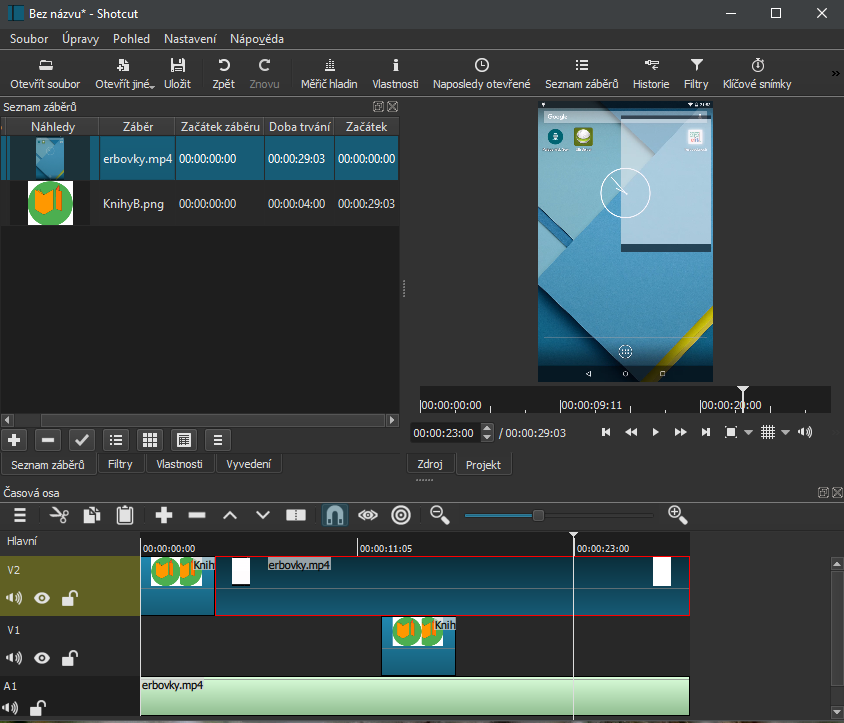
\includegraphics{obrazky-figures/shotcup.png}
	}
	\caption{Uživatelské rozhraní nelineárního video editoru Shotcut.}\label{img:shotcut}
\end{figure}

Bezplatnou aplikací nevyužívající framework MLT je například program \textit{Openshot}\,\footnote{Openshot -- bezplatný nelineární editor s~prostředím GTK+, \url{https://www.openshot.org/}.}, který přešel na vlastní jádro. Jeho rozhraní je oproti předchozím dvou editorům velmi zjednodušené. Rozvržení zůstává stejné, pouze omezuje počet informací, které uživateli poskytuje. Nahoře se opět nacházejí akce k~projektu, vlevo knihovna souborů, filtrů a přechodů, vpravo náhled s~jednoznačnými ikonami a ve spodní části se nacházejí časové osy a rovněž se zde nastavují vlastnosti filtrů/přechodů. I~přes zjednodušení rozhraní zde žádné funkce nechybí.

Mezi kvalitní proprietární programy se řadí program \textit{iMovie} od firmy Apple, \textit{Adobe Premiere Pro} od firmy Adobe Systems a \textit{VEGAS Movie Studio} od firmy Sony. Profesionální programy se od bezplatných liší zejména vyšší stabilitou, propracovanějšími filtry a šablonami. Licence se pohybují v~řádech tisícikorun a například Adobe nabízí svůj produkt pouze ve formě předplatného. Z~těchto programů jsem vyzkoušel \textit{iMovie}. Program od firmy Apple dělí pracovní prostor do stejných skupin. Na rozdíl od předešlých programů zobrazuje v~levé polovině nejen soubory k~aktuálnímu projektu, ale i soubory v~knihovnách. V~navrhovaném řešení je rovněž potřeba řešit sdílenou knihovnu s~obecnými zdroji sdílenými například s~uživateli fakulty. Odlišná je aplikace filtrů. Filtry se nacházejí nad náhledem videa, jako ikony pro skupiny filtrů. Po rozkliknutí ikony se zobrazí nabídka filtrů. Uživatel nikdy nenastavuje číselné hodnoty. Nastavení filtrů je řešeno vizuálními posuvníky, kapátky a dalšími nástroji. Zajímavě řešená je časová osa, která nemá pravítko s~časem. Měřítko času je na ose proměnlivé, obrázek \ref{img:imovie}. Mezi klipy je mezera, ačkoliv konec předchozího a začátek následujícího klipu je ve stejný čas. Z~mého pohledu se jedná o~rušivý prvek, při přehrávání ukazatel aktuálního času přeskakuje a mění svou rychlost. Na druhou stranu lze do mezer pohodlně vkládat přechody. Za zvláštní vlastnost považuji nemožnost posouvat položky po časové ose, je možné pouze měnit pořadí položek. Pokud potřebujeme mít ve videu prázdné místo, musíme zde vložit jednolitou barvu z~knihovny (záložky Pozadí). Nad časovou osou chybí lišta nástrojů. Nástroje k~položkám časové osy jsou dostupné skrze kontextovou nabídku vyvolanou stiskem pravého tlačítka myši nebo skrze klávesové zkratky. Video stopy jsou laděny do modrých barev, zvukové stopy do barev zelených. Z~programu iMovie jsem čerpal tmavé barevné schéma.
\begin{figure}[h]
	\centering
	\scalebox{0.3}{
		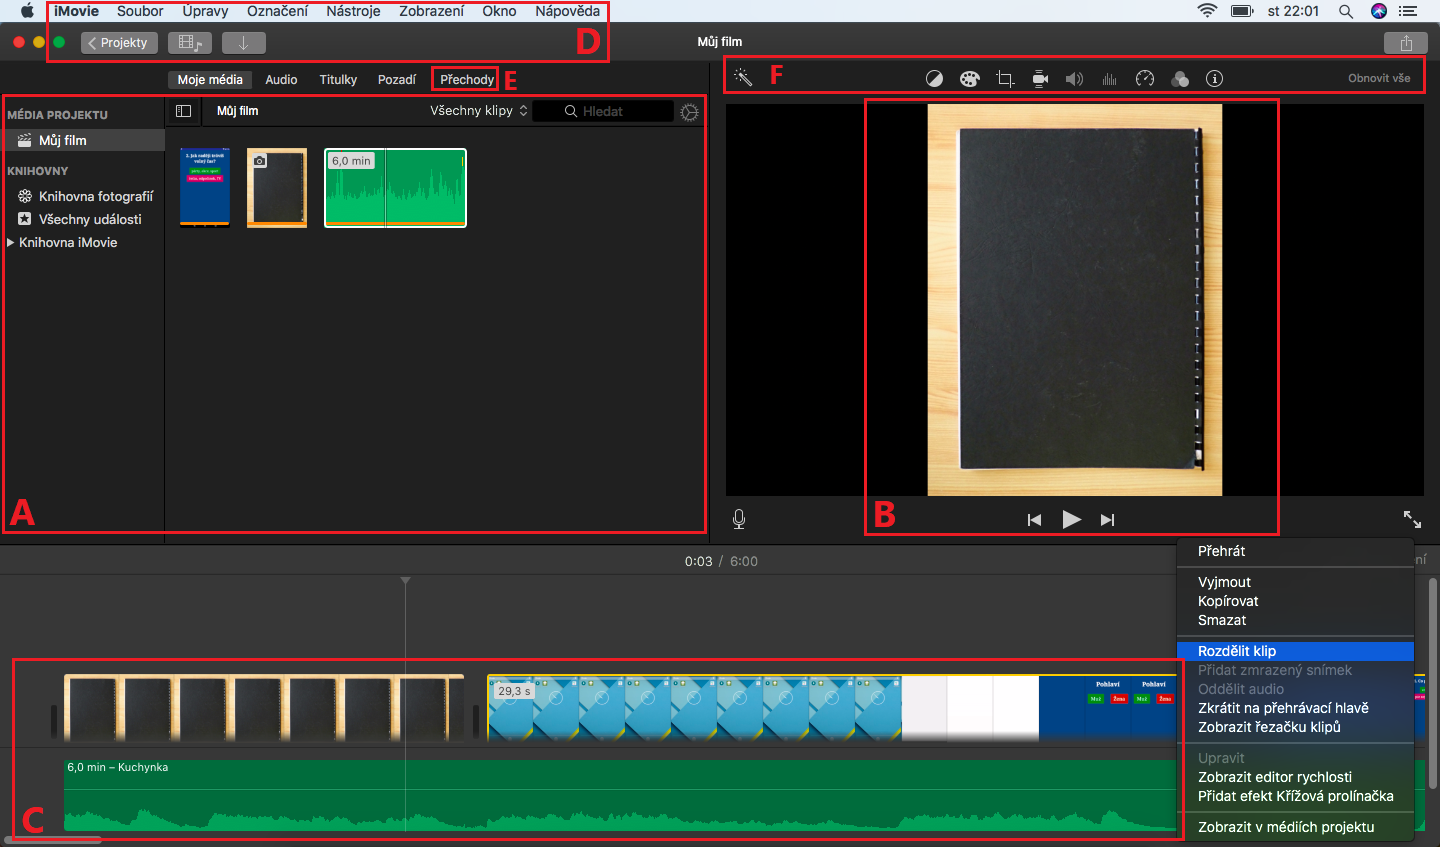
\includegraphics{obrazky-figures/iMovie.png}
	}
	\caption{Uživatelské rozhraní iMovie. Časová osa nemá jednotné měřítko.}\label{img:imovie}
\end{figure}

Zajímavým projektem mezi desktopovými aplikacemi je open source editor \textit{fwf}\,\footnote{fwf -- JavaScriptový FFmpeg editor, \url{https://github.com/daem-on/fwf}.} -- lineární video editor využívající knihovnu \textit{FFmpeg}\,\footnote{FFmpeg -- multiplatformní řešení pro nahrávání, konverzi a streamování audia a videa, \url{https://ffmpeg.org/}.}. Program je napsaný v~JavaScriptovém frameworku \textit{Vue.js}\,\footnote{Vue.js -- open source JavaScriptový framework pro tvorbu uživatelských rozhraní, \url{https://vuejs.org/}.} a zkompilovaný pomocí nástroje \textit{Electron}\,\footnote{Electron -- nástroj pro tvorbu desktopových aplikací za pomocí JavaScriptu, HTML a CSS, \url{https://electronjs.org/}.}. Video editor má pouze základní funkce, není příliš spolehlivý, ale lze se u~něj inspirovat s~použitými technologiemi pro implementaci uživatelského rozhraní, obrázek \ref{img:fwf}.
\begin{figure}[h]
	\centering
	\scalebox{0.4}{
		\includegraphics{obrazky-figures/fwf.png}
	}
	\caption{Uživatelské rozhraní editoru \textit{fwf}, sestavené nástrojem Electron.}\label{img:fwf}
\end{figure}
Na časovou osu jsem použil knihovnu \textit{vis.js}\,\footnote{vis.js -- JavaScriptová knihovna na vizualizaci dat, \url{http://visjs.org/}.}. \textit{Timeline} je jen jedním z~vizualizačních nástrojů knihovny. Knihovna slouží k~zobrazení událostí od Unixové epochy (00:00:00,000 1. ledna 1970), zatímco projekt začíná časem 0. Dále jsem z~projektu použil font Source Sans Pro zveřejněnou pod svobodnou Open Font Licencí a pro ikony odnož\,\footnote{Material Design Icons -- odnož projektu Google, \url{https://github.com/jossef/material-design-icons-iconfont}.} použitého fontu Material Icons od Google (licence Apache-2.0).

\section{Webové editory}
Na webový editor jsem nezískal žádný tip. Lidé v~mém okolí raději sáhli po open source editoru či stáhli placený program obsahující crack pomocí torrentu. U~webových editorů je velký rozdíl mezi placenými řešeními a neplacenými. Placených aplikací je nepřeberné množství s~mnoha funkcemi, bezplatná řešení mají zásadní omezení. Řešení s~otevřeným zdrojovým kódem a svobodnou licencí jsem nenašel žádné.

Placená řešení se funkcemi i rozhraním blíží nativním aplikacím. Z~placených editorů zmiňuji \textit{WeVideo}\,\footnote{WeVideo --  proprietární online editor, \url{https://www.wevideo.com}.}, \textit{Magisto}\,\footnote{Magisto -- proprietární online editor, \url{https://www.magisto.com/}.}, \textit{Loopster}\,\footnote{Loopster -- proprietární online editor, \url{https://www.loopster.com}.}, \textit{Animatron}\,\footnote{Animatron -- proprietární online editor s~nejdražším předplatným, \url{https://www.animatron.com}.} a \textit{Clipchamp}\,\footnote{Clichamp Create -- proprietární online editor, který lze používat s~omezeními bezplatně, \url{https://clipchamp.com}.}.

\textit{WeVideo} je poskytováno v~mnoha plánech. Nejdražší varianta neomezuje velikostí souboru ani maximální délkou. Uživatelské rozhraní umožňuje pracovat s~video soubory již během nahrávání na server. Náhled je renderován v~prohlížeči, výsledné video na serveru. Po dokončení renderování je uživateli zaslán email. Videa vytvořená v~bezplatném plánu obsahují vodoznak.

\textit{Magisto} nabízí pouze placené plány. Nejlevnější plán limituje maximální délkou výsledného videa 2,5 minuty. Nejdražší plám má rovněž velmi limitující omezení -- 10 minut.

\textit{Loopster} nabízí ve všech plánech výstupní rozlišení 1080p. Zásadním problémem pro zpracovávání přednášek je maximální délka -- 30 minut u~nejdražšího plánu.

\textit{Animatron} slouží spíše k~tvorbě krátkých upoutávek a reklam. Umožňuje v~nejdražším předplatném vytvořit projekt o~maximální délce 10 minut. Bezplatný plán neumožňuje stažení videa, pouze vystavení videa na sociálních sítích. Při práci s~editorem jsem zaznamenal problém s~různou orientací stejného videa napříč editorem.

Pro nenáročné uživatele by mohl být dostačující nástroj \textit{Clipchamp Create}, který nabízí i bezplatný plán s~omezením rozlišení videí na 480p. Velikost projektu omezena není a video není opatřeno reklamním vodoznakem. Rozhraní je shodné s~desktopovými programy, obrázek \ref{img:clipchamp}. Editor běží pouze v~prohlížeči Google Chrome a zpracování videa probíhá na straně webového prohlížeče. Uživatel nesmí videoeditor během zpracovávání opustit. Doba zpracování videa o~délce do 2 minut trvá i při rozlišení 480p cca 20 minut.
\begin{figure}[h]
	\centering
	\scalebox{0.5}{
		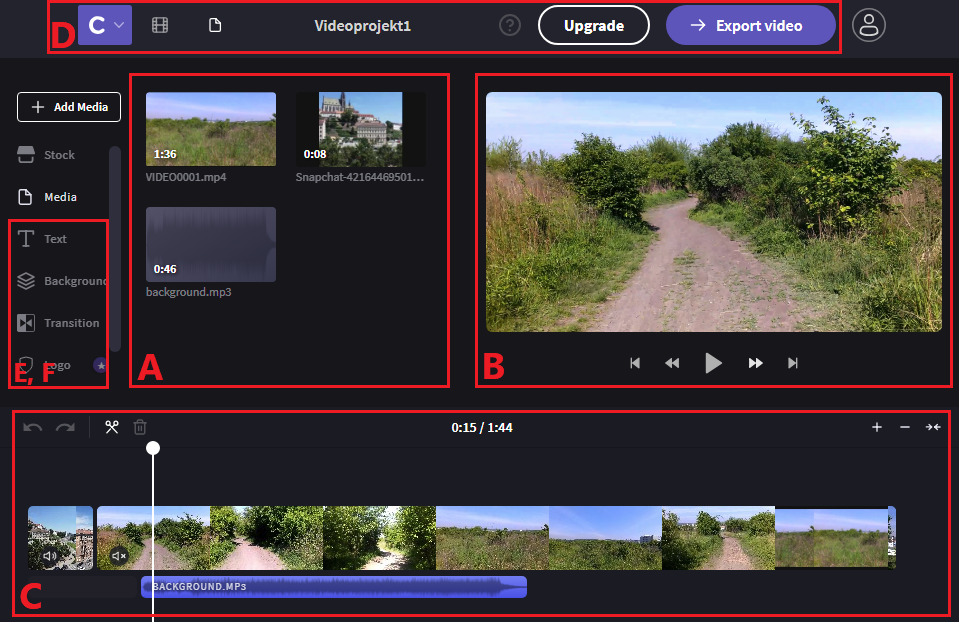
\includegraphics{obrazky-figures/clipchamp.png}
	}
	\caption{Uživatelské rozhraní nelineárního online video editoru \textit{Clipchamp Create}.}\label{img:clipchamp}
\end{figure}

Další dva editory uvádím pro úplnost, ani jeden není použitelný -- \textit{Kizoa}\,\footnote{Kioza -- bezplatný lineární online video editor, \url{https://www.kizoa.com}.} a \textit{Movie Maker Online}\,\footnote{Movie Maker Online -- bezplatný online editor, \url{https://moviemakeronline.com/}.}.

Editor \textit{Kizoa} je vytvořen v~programu \textit{Adobe Flash}, obsahuje dostatečné množství efektů, přechodů a nastavení. Vespod zobrazuje jednu časovou osu, jedná se o~lineární editor. Hlavní nevýhodou je vázanost na \textit{Adobe Flash Player}, který je dnes na ústupu a jeho podpora skončí v~roce 2020\,\cite{FlashPlayer}. Bezplatné předplatné nabídne 2 minuty videa s~rozlišením 720p, nejdražší předplatné 4K video bez omezení délky.
\begin{figure}[h]
	\centering
	\scalebox{0.53}{
		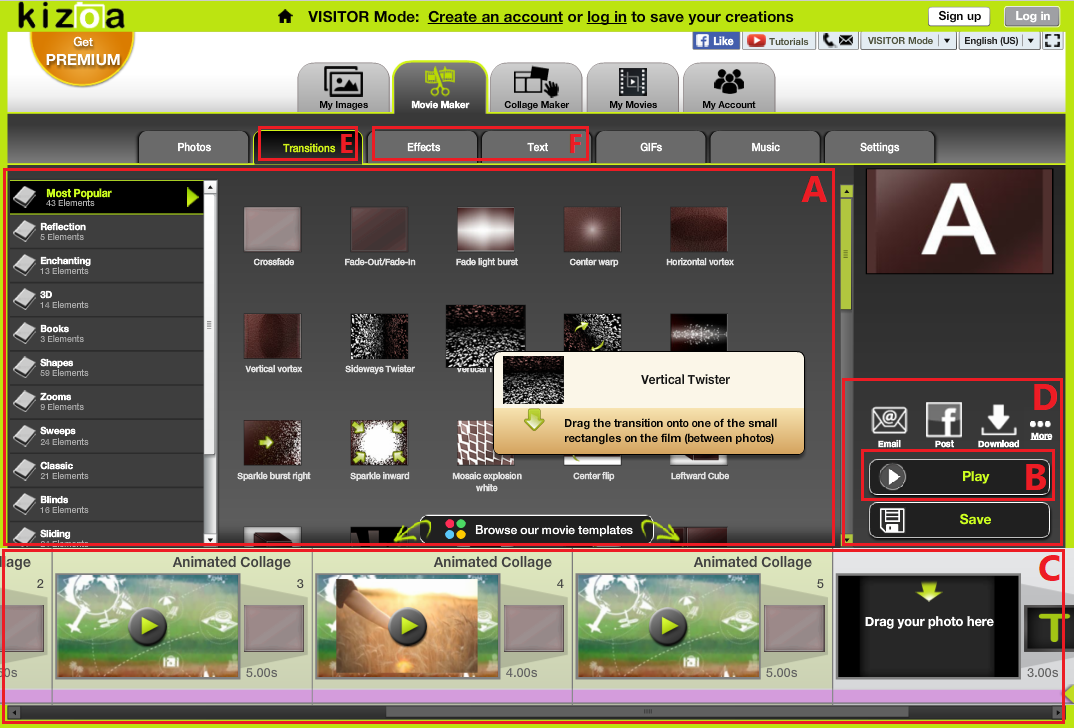
\includegraphics{obrazky-figures/kizoa.png}
	}
	\caption{Uživatelské rozhraní online lineárního video editoru Kizoa.}\label{img:kizoa}
\end{figure}

\textit{Movie Maker Online} představuje video editor s~netradičním uživatelským rozhraním. Nevyužívá zásuvných modulů a osu s~videem zobrazuje vertikálně. Jedná se o~nelineární editor, který má 4 stopy -- zvukovou, stopu s~pozadím, hlavní stopu a stopu s~překryvným textem. Přidat nebo odebrat stopu není možné. Editor je řešen jako jedna stránka, na které se pod sebou nacházejí jednotlivé kroky. Nahrávání souborů probíhá v~prvním kroku, poté se musí uživatel přesunout ke kroku 2 a provést editace. Pro uživatele desktopových aplikací se jedná o~zcela jiné rozhraní, ve kterém se budou těžko orientovat. Na rozdíl od předchozího řešení neumožňuje \textit{Movie Maker Online} projekt uložit nebo exportovat a později opětovně použít. Program lze používat bez registrace, výsledné video o~rozlišení 720p je opatřeno vodoznakem a nesmí přesáhnout 10 minut. Program by měl nabízet předplatné, aktuálně ale nelze získat.
\begin{figure}[h]
	\centering
	\scalebox{0.53}{
		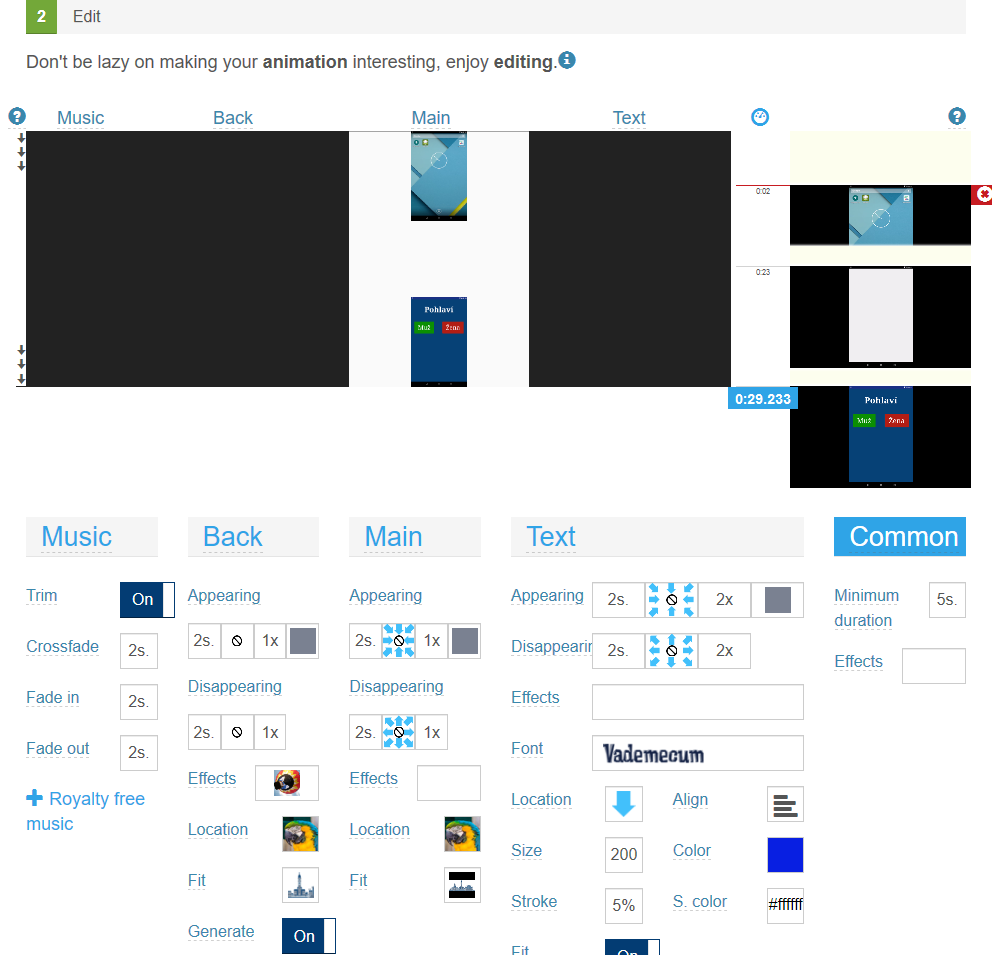
\includegraphics{obrazky-figures/moviemakeronline.png}
	}
	\caption{Uživatelské rozhraní online video editoru Movie Maker Online.}\label{img:moviemakeronline}
\end{figure}

\section{Shrnutí}
U~desktopových aplikací máme široký výběr. Všechny testované programy mají podobný způsob ovládání i podobné funkce. Nemusíme se bát sáhnout po bezplatném open source řešení, i tyto programy obsahují dostatek funkcí pro kvalitní tvorbu. Neobsahují omezení na maximální rozlišení nebo délku výsledného videa. Dražší programy nabídnou propracovanější filtry a vyšší stabilitu. Při návrhu online videoeditoru je dobré zachovat rozhraní, které uživatelé znají právě z~těchto aplikací. Z~pohledu technologií je zajímavý jednoduchý open source lineární editor \textit{fwf}, který je napsán v~JavaScriptovém framoworku \textit{Vue.js}.

Webových řešení je rovněž široký výběr. Mezi jednotlivými aplikacemi je velký rozdíl ve funkcích a zejména v~omezeních výsledného videa. Z~testovaných řešení nabízí neomezenou délku videa pouze program \textit{WeVideo}, \textit{Clipchamp Create}, který ale zpracovává videa v~prohlížeči a \textit{Kizoa}, kterého jsem vyřadil ze srovnání kvůli vázanosti na \textit{Adobe Flash}. V~rozhraních jsou větší rozdíly než u~desktopových aplikací. Uživatel desktopových editorů videa nebude mít problém s~orientací v~jednom z~online editorů, vyjma \textit{Movie Maker Online} se zcela odlišným rozhraním. Nabízených tarify a zásadní omezení online videoeditorů srovnávám v~tabulce \ref{tab:prices}.

V~případě, že požadujeme online editor videí, ale zároveň potřebujeme mít svá data pod kontrolou na svém serveru, připadá v~úvahu pouze program \textit{Clipchamp Create}. Program provádí veškeré operace přímo v~prohlížeči. Renderování delších videí s~rozlišením větší než 480p vyžaduje výkonný hardware. V~tomto případě je lepší sáhnout po desktopové aplikace. Pokud chceme zpracovávat videa online, ale na našem serveru, máme smůlu.

\begin{table}[h]
    \centering
    \begin{tabular}{|l|l|l|}
    \hline
    Program   & Magisto & Animatron\\
    \hline
    Plány   & 480p, 2,5 min 230 Kč & 720p, 15 s~0 Kč\\
            & 720p, 10 min 461 Kč   & 720p, 1 min 230 Kč\\
            & 1080p, 10 min 1614 Kč & 1080p, 5 min 899 Kč\\
            &                       & 1080p, 10 min 1360 Kč\\
    \hline
    Pozn.   & Měsíční i roční předplatné. & Měsíční i roční předplatné.\\
    \hline
    \hline
    Program & Loopster                                  & WeVideo\\
    \hline
    Plány   & 1080p, 20 min, 10 GB 115 Kč               & 480p, 5 min/měs., 1 GB, 0 Kč\\
            & 1080p, 30 min, 20 GB 230 Kč               & 720p, 30 min/měs., 20 GB, 230 Kč\\
            & 1080p, 30 min, 100 GB 2975 Kč / 3 měs.    & 4K, neomezeno 369 Kč\\
            &                                           & 4K, 3 uživ. 1383 Kč + 922 Kč/uživ.\\
    \hline
    Pozn.   & Roční předplatné.                         & Měsíční i roční předplatné.\\
            & Poslední plán účtován čtvrtletně.         & Poslední plán je multilicence.\\
    \hline
    \end{tabular}
    \caption{Přehled tarifů placených online video editorů. Pokud není uvedeno jinak, cena je za měsíc. Videa delší než 30 minut nabízí pouze WeVideo.}
    \label{tab:prices}
\end{table}

\chapter{Návrh řešení}
Hlavním cílem práce je vytvořit videoeditor, který bude fungovat ve všech moderních prohlížečích a výsledné zpracování videa nebude probíhat na straně klienta. K~dosažení těchto cílů bude za nutné vytvořit webovou aplikaci. Stejně jako stávající řešení by i tento editor měl provádět veškeré úkony pomocí JavaScriptu a asynchronních požadavků, bez nutnosti znovu načítat celou stránku. Vzhledem ke komplexnosti uživatelského rozhraní není vhodné zvolit čistý JavaScript. Vyplatí se sáhnout po JavaScriptovém frameworku, usnadňují časté operace, udržují dobré návyky a pomáhají vytvořit čistý kód.

Nejpoužívanějšími frameworky jsou: React, Backbone.js, RequireJS, AngularJS, nebo třeba Vue.js (používané programem \textit{fwf})\,\cite{WappalyzerJavasript}. Z~těchto frameworků jsem vybral React, který je zároveň i šablonovacím systémem a má kvalitní dokumentaci. Šablonovací systém používám zejména k~rozdělení uživatelského rozhraní na komponenty.

Webová aplikace bude potřebovat i serverovou část, na kterou klient nahraje soubory, popíše serveru operace nad soubory a dá pokyn pro vyhotovení výsledného videa. Tuto architekturu označujeme z~pohledu sítě jako klient-server. Z~pohledu návrhu se bude jednat o~MVC (model-view-controller) architekturu. Mezi klientem a serverem je nutné komunikovat. Pro výměnu dat po síti musejí obě části používat dohodnutý serializační formát. JavaScript nejčastěji používá \textit{XML} nebo \textit{JSON}. \textit{JSON} (JavaScriptový objektový zápis) je novější a zápis ve formátu \textit{JSON} je validním kódem JavaScriptu. \textit{XML} (rozšiřitelný značkovací jazyk) na druhou stranu umožňuje přenos binárních dat. Se serverem bude komunikovat JavaScript, volba formátu \textit{JSON} je tedy výhodná.

Sever bude mít za úkol 2 činnosti. Nejprve bude muset uživateli poskytnout soubory s~HTML, CSS a JavaScriptem a poté reagovat na JavaScriptové asynchronní požadavky. Při návrhu jsem se rozhodoval mezi implementací serveru pomocí jazyka PHP a pomocí Node.js. Jazyk PHP vznikal v~době statických stránek a osobních webů, Node.js je obvykle spojován se single page aplikacemi. Node.js jsem si vybral právě protože plánuji vytvořit single page aplikaci, kvůli možnosti používat stejný jazyk pro klientskou i serverovou část a také kvůli asynchronnímu přístupu k~blokujícím operacím. Po PHP bych naopak sáhl při tvorbě e-shopu, blogu či informačního systému.

Server bude pro klienta dostupný skrze rozhraní (API). Rozhraní bude sloužit k~vyvolání akcí na serveru i k~získávání dat. Existuje více koncepcí pro komunikaci a tvorbu API, například \textit{XML-RPC}, \textit{SOAP} nebo \textit{REST}. \textit{XML-RPC} a \textit{SOAP} používají jako serializační formát pro výměnu dat \textit{XML}, kvůli JavaScriptu na straně klienta i serveru jsem ovšem zvolil \textit{JSON}. \textit{REST} je způsob komunikace na základě HTTP požadavků. \textit{REST} není na HTTP vázaný, ale není praktický důvod používat odlišný protokol. Výchozím serializačním formátem pro výměnu dat je JSON, ovšem lze používat například i \textit{XML}.

Multimediální soubory bude potřeba zpracovávat. \textit{Clipchamp Create} provádí zpracování na straně klienta ve webovém prohlížeči. Webový prohlížeč ani webové technologie ale nejsou navrženy na renderování videí, \textit{Clipchamp} vyvádí video déle, než bych byl ochotný čekat. Editor byl navržen, aby zpracovával videa na serveru. K~tomu může sloužit program \textit{FFmpeg} nebo \textit{MLT}. Program \textit{FFmpeg} používá například editor \textit{fwf} nebo Android aplikace \textit{Video Editor using FFmpeg}\,\footnote{Video Editor using FFmpeg -- open source editor videa pro android, \url{https://github.com/bhuvnesh123/FFmpeg-Video-Editor-Android}.}. \textit{FFmpeg} se používá skrze příkazový řádek. Každá operace představuje jeden příkaz (zkrátit video, přidat efekt, spojit videa). Na pořadí operací záleží. Projekt by byl popsán souborem s~posloupností příkazů pro FFmpeg, případně jedním dlouhým příkazem. Multimediální framework \textit{MLT} rovněž nabízí své nástroje skrze příkazový řádek. Projekt je možné popisovat posloupností příkazů a také pomocí serializačního formátu \textit{XML}. Celý projekt se popíše entitami \textit{XML} a programu \textit{MLT} se poté pouze předá \textit{XML} sobor. \textit{XML} soubor bude uložen po celou dobu na serveru a server jej bude editovat na základě požadavků klienta. \textit{REST API} je bezstavové, požadavek musí být úplný a stav projektu je uložen v~\textit{XML} souboru projektu. Projekt nebude využívat databázového systému.

Seznam použitých technologií, jejich umístění a komunikaci zobrazuje obrázek \ref{img:server-architektura}.
\begin{figure}[h]
	\centering
	\scalebox{0.6}{
		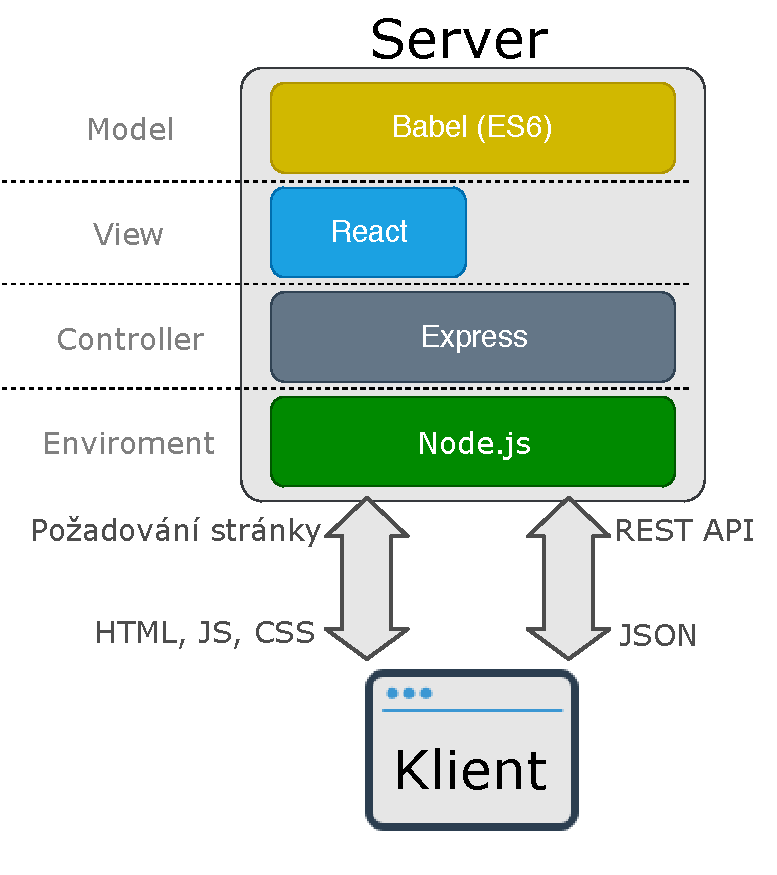
\includegraphics{obrazky-figures/server-architektura.pdf}
	}
	\caption{Architektura serveru.}\label{img:server-architektura}
\end{figure}

\section{Zvolené technologie}
\subsection{Node.js}
Node.js vytváří běhové prostředí JavaScriptu postavené na JavaScriptovém enginu V8 od firmy Google. Umožňuje používat JavaScript jako systémový jazyk, který má přístup k~paměti, bufferům, procesům, souborům a soketům. Cílem Node.js je poskytovat snadnou cestu k~vytvoření škálovatelných síťových aplikací. Node.js nepoužívá vlákna, je založen na událostech a asynchronním vykonávání blokujících operací, umožňuje snadnou modularitu. Právě eliminací blokujících operací pomocí asynchronní obsluhy řízenou událostmi lze dosáhnout vysokého výkonu. PHP vytváří pro každý požadavek samostatné vlákno a v~případě blokující operace čeká na vyřízení, Node.js používá pro všechny požadavky jedno vlákno a namísto paralelního zpracování používá Node.js pseudoparalelní zpracování.

Pro porovnání rychlosti vykonání programu, uvedu příklad jednoduchého programu, ve kterém se v~prázdném cyklu inkrementuje miliardkrát čítač. Doba běhu programu je pro jednotlivé jazyky následující -- JavaScript (Node.js verze 9.3.0) 0,635 sekund, jazyk C (Apple LLVM 8.1.0) 2,398 sekund a Python (3.6.1) 31,096 sekund. Všechny testy probíhaly na zařízení MacBook Pro s~procesorem Intel Core i7 2,8 GHz. Překladač V8 JavaScript kompiluje namísto interpretování, díky tomu lze využívat vysokoúrovňový jazyk bez nutnosti vzdát se rychlosti kompilovaných jazyků\,\cite{MasteringNodejs}.

JavaScript na klientské straně je pro interaktivní webovou aplikaci nutnost. Díky běhu JavaScriptu na klientské i serverové části mohou programátoři používat jeden jazyk v~rámci projektu. Dále se otevírá možnost používat stejný kód na serveru i na straně klienta. Stačí vhodně členit funkce do modulů a tyto moduly poté importovat jak na straně serveru, tak na straně klienta. V~mé práci takto sdílím kód pro práci s~časovými značkami.

\subsection{Express framework}
Pro usnadnění tvorby webového serveru jsem použil Express. Express je webový framework pro Node.js. Poskytuje knihovny užitečné pro zajištění základních funkcí webového serveru (routování, podpora šablonovacího systému pro generování stránek, zpracování dotazů, parametrů, sezení a cookies, autentifikaci, vytváření odpovědí, zpracování chyb, aj.).

\subsection{ECMAScript, TypeScript}
Jedná se o~programovací jazyk se syntaxí inspirovanou jazykem C, který se překládá do JavaScriptu. TypeScript je nadstavba nad JavaScriptem, program v~JavaScriptu je validním programem v~TypeScriptu. Přináší silnou typovou kontrolu, třídy (dnes i v~ES6), rozhraní, dědičnost. Offline překlad do JavaScriptu odhalí syntaktické chyby, a volitelně zajistí kompatibilitu se standardy ES3 a ES5 (alternativou je \textit{Babel}, na kontrolu kódu na syntaktické chyby pak \textit{ESLint}\,\footnote{ESLint -- nástroj pro analýzu JavaScriptového kódu, \url{https://eslint.org/}.}). Dále přidává spoustu \uv{syntaktického cukru} -- gettery/settery, výčtové typy, promises. Podporuje integraci s~Angular 2 i React.

Na druhou stranu je typová kontrola plnohodnotná pouze pokud všechny balíčky obsahují hlavičkové soubory TS. TypeScript je nutné začlenit do vývojového procesu s~Node.js a React. Během vývoje se při každé změně zdrojového kódu musí provést kompilace do JavaScriptu. Pro začínajících programátory a pro malé projekty zavádí složitost, která nemusí převážit výhody zavedení.

S~příchodem ES6 přejal standard z~TypeScriptu deklaraci proměnných s~platností v~daném rámci bez vedlejších efektů (\texttt{let}), možnost vytvářet třídy, dědičnost, rest parametry, promises a další. Hlavní výhodou zůstává silné typování a kontrola syntaxe při kompilaci. Vzhledem k~mým předchozím zkušenostem s~jazykem PHP jsem tyto vlastnosti nepožadoval, proto jsem se rozhodl použít standard ES6 a novější revize. Zpětnou kompatibilitu klientského JavaScriptu jsem zajistil nástrojem \textit{Babel}.

\subsection{React}
React je JavaScriptová knihovna pro tvorbu uživatelských rozhraní. Je založen na komponentách, stavech komponent a na signálech mezi komponentami. Knihovna dovolí rozdělit uživatelské rozhraní do od sebe izolovaných částí kódu -- komponent. Každá komponenta má svůj vlastní stav, své funkce a má plně pod kontrolou své vykreslení. Vztah komponent bývá hierarchický, skládáním komponent můžeme vytvořit komplexní rozhraní při zachování čistého kódu. Stav aplikace uchovávají jednotlivé komponenty, stav má jedno centrální úložiště. Někdy nám tato vlastnost nemusí vyhovovat. V~takovém případě stačí vytvořit kořenovou komponentu, a původní komponenty vložit do kořenové komponenty. Úložištěm stavu poté může být kořenová komponenta. Jak může vypadat komponenta React ukazuje následující ukázka.
\begin{lstlisting}[style=JavaScript]
import React, { Component } from 'react';
import SourcesTableRow from './SourcesTableRow';
import Uploader from './Uploader';

export default class Sources extends Component {
    constructor(props) {
        super(props);
        this.delResource = this.delResource.bind(this);
        this.putResource = this.putResource.bind(this);
    }
    render() {
        return (
            <div id={'sources'}>
                <i className="material-icons" aria-hidden="true">video_library</i>
                <table>
                <tbody>
                    {Object.keys(this.props.items).map(key =>
                        <SourcesTableRow
                            key={this.props.items[key].id}
                            item={this.props.items[key]}
                            onRemove={this.delResource}
                            onInsert={this.putResource}
                        />)
                    }
                    <tr>
                        <td colSpan="3">
                        <Uploader value={{
                            onAdd: resource => this.props.onAddResource(resource),
                            project: this.props.project,
                        }}
                        />
                        </td>
                    </tr>
                </tbody>
                </table>
            </div>
        );
    }
    ...
\end{lstlisting}

Na ukázce je vidět hierarchie komponent. Aktuální komponentou je \texttt{Sources}, komponenta se v~těle funkce pro vykreslení odkazuje na \texttt{SourcesTableRow} a \texttt{Uploader}. Komponenta \texttt{Sources} bude těmto dvěma komponentám nadřazená. Pokud by byla komponenta \texttt{Sources} kořenová, nemá na ni kdo odkazovat. Je potřeba určit v~jakém místě HTML stránky se má vykreslit. Toho docílíme v~JavaScriptovém souboru, který Webpack zkompiluje do klientského JavaScriptového souboru:
\begin{lstlisting}[style=JavaScript]
ReactDOM.render(<Sources items={{}} onAddResource={() => {}} />, document.getElementById('app'));
\end{lstlisting}

Pokud uživatel navštíví stránku s~React komponentami, získá nejprve soubor HTML s~kostrou stránky. Vespod HTML bude odkaz na JavaScriptový soubor, který se stáhne, vykoná a nahradí elementy kostry s~vykreslenými React komponentami. V~tomto případě se obsah elementu \texttt{ <div id="{}app"{}></div>} nahradí vykreslenou komponentou \texttt{Sources}.
\begin{lstlisting}[language=HTML]
<!DOCTYPE html>
<html lang="cs" dir="ltr">
    <head>
        <title>React page</title>
    </head>
    <body>
        <div id="app">
            <h2>Nacitani<h2>
            Pokud se aplikace nenacte, zkontrolujte zapnuty JavaScript
        </div>
        <script src="/main.js" async></script>
    </body>
</html>
\end{lstlisting}

Pokud má být výsledný kód přehledný, vyplatí se vytvářet komponenty jako třídu, která rozšiřuje třídu \texttt{Component}. Je vhodné pro každou třídu použít samostatný soubor a třídu s~komponentou určit jako výchozí export. Díky tomu můžeme ostatní komponenty použít importem souboru.

Třída komponenty může obsahovat vlastní funkce a také funkce, které mají zvláštní význam. Funkce konstruktoru třídy (\texttt{constructor}) je obvyklá. Na začátku konstruktoru musíme volat konstruktor předka. V~konstruktoru se obvykle nastavuje stav komponenty, atributy třídy a také se zde fixuje kontext pro proměnnou \texttt{this} uvnitř funkcí. Pokud totiž funkce předáme jiné komponentě v~parametrech (jako callback) a funkci zavoláme z~jiné komponenty, bude \texttt{this} odkazovat na komponentu, ze které volání vychází. Metoda \texttt{bind} tomuto nechtěnému chování zabrání.

Dalšími důležitými metodami zvláštního významu jsou například: \texttt{render}, \texttt{componentDidMount}, \texttt{componentDidUpdate} a \texttt{componentWillUnmount}.

Metoda \texttt{render} zajišťuje vykreslení komponenty. Funkce za úkol vrátit JSX kód komponenty. JSX je rozšíření syntaxe JavaScriptu. JSX svou syntaxí připomíná spíše XML, než HTML. Všechny tagy jsou párové (musejí být uzavřeny). Kód musí být uzavřen do kořenového elementu. Pokud nechceme vykreslovat žádný kořenový element, můžeme použít elementy s~prázdnými tagy \texttt{<></>}. JSX kombinuje HTLM a JavaScript. Příkazy a proměnné JavaScriptu jsou dostupné ve složených závorkách -- \texttt{\{this.props.items\}}. Atributy HTML prvků se zapisují v~CamelCase (notaci velkých písmen). Atributy nabývají stejných hodnot, jako JavaScriptové proměnné. Zvláštností je atribut \texttt{style}, který přijímá objekt s~CSS vlastnostmi\,\cite{jsx}.

Zbývající metody se volají při vložení komponenty do virtuálního DOM stromu, který si React vytváří, při aktualizaci a při odstraňování z~DOM.

Aby uživatelské rozhraní fungovalo, musejí mezi sebou komponenty komunikovat. Komponenty mají stromovou strukturu, komunikace probíhá dvěma směry -- od předka k~potomkovi a naopak. Komponenty mohou podřazeným komponentám při jejich vytváření předat parametry. Můžeme předávat callbacky nebo stav komponenty. V~podřazené komponenty jsou tyto parametry dostupné skrze objekt \texttt{this.props}. Pokud podřazené komponentě předáme stav a podřazená komponenta se stavem přímo pracuje ve funkci \texttt{render}, dojde se změnou stavu předka i k~aktualizaci a překreslení podřazené komponenty. Pokud například změníme stav kořenové komponenty, může tato změna \uv{probublat} ke komponentám o~několik úrovní níže, vše se děje automaticky. Komunikace směrem ke kořeni probíhá pomocí callbacků. Podřazená komponenta může změnit stav nadřazené pouze nepřímo. Zavolá funkci, kterou mu nadřazená komponenta zpřístupnila v~\texttt{this.props}, na základě volání nadřazená komponenta změní svůj stav a obě komponenty se překreslí.

Stav komponenty se nastavuje metodou \texttt{this.setState}. Jako parametr se předá objekt s~položkami, které se mají přepsat. Předchozí a následující stav se nesmí ovlivňovat. Pokud chceme upravit jen jednu položku objektu, musíme vytvořit kopii objektu a tuto kopii nastavit jako nový stav\,\cite{react}.

\section{Návrh uživatelského rozhraní}
Cílovou skupinou jsou počítačově gramotní uživatelé, kteří někdy používali program na editování videa. Rozhraní je voleno tak, aby připomínalo klasické desktopové aplikace a pomohlo uživatelům se zorientovat. Typickou úlohou pro videoeditor bude sestříhat záznam přednášky do výukového videa nebo vytvořit tutoriál ze záznamu z~kamery nebo obrazovky. Aplikace bude využívána na počítačích a noteboocích, není nutné přizpůsobovat rozhraní obrazovkám mobilních zařízení. Ovládání bude pomocí klávesnice a myši, dotekové obrazovky se sice nepředpokládají, ale ani nevylučují.

Po načtení hlavní stránky se zobrazí úvodní stránka s~možností vytvořit nový projekt. Stránka bude do budoucna připravena na rozšíření o~další možnosti, jako jsou šablony, autentizace uživatelů, či seznam vlastních projektů. Pro zahájení editace uživatel zvolí \textit{Vytvořit nový projekt}, obrázek \ref{img:novy-projekt}.
\begin{figure}[h]
	\centering
	\scalebox{0.5}{
		
\includegraphics{obrazky-figures/novy_projekt.png}
	}
	\caption{Úvodní obrazovka pro vytváření nových projektů.}\label{img:novy-projekt}
\end{figure}

Po vytvoření nového projektu se uživatel ocitne v~rozhraní pro tvorbu videí. Aplikace je řešena jako single page aplikace. Uživatel po celou dobu pracuje na jedné obrazovce a i při dialozích je editor překryt pouze částečně, tak, aby měl uživatel pocit, že má svůj projekt po celou dobu pod kontrolou. Při návrhu uživatelského rozhraní editoru jsem se nejvíce inspiroval desktopovou aplikací \textit{iMovie}, \textit{Shotcut} a online nástrojem pro úpravu fotografií -- \textit{Photopea}\,\footnote{Photopea.com -- bezplatný editor fotografií, \url{https://www.photopea.com/}.}.

Uživatelské rozhraní editoru je rozděleno do 4 částí. Rozložení bylo navrženo a odzkoušeno na drátěném modelu, obrázek \ref{img:wireframe}.
\begin{figure}[h]
	\centering
	\scalebox{0.3}{
		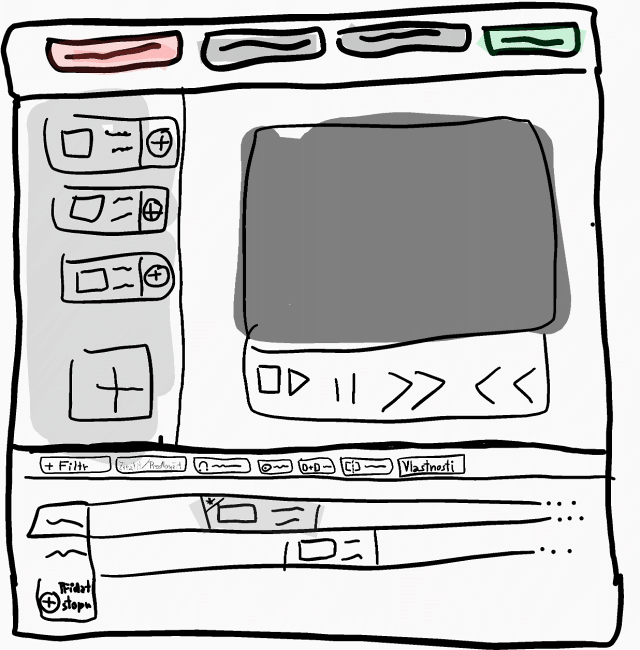
\includegraphics{obrazky-figures/wireframe}
	}
	\caption{Drátěný model uživatelského rozhraní.}\label{img:wireframe}
\end{figure}
Na základě drátěného modelu byl zhotoven prototyp hlavního uživatelského rozhraní, obrázek \ref{img:mockup}.
\begin{figure}[!h]
	\centering
	\scalebox{0.6}{
		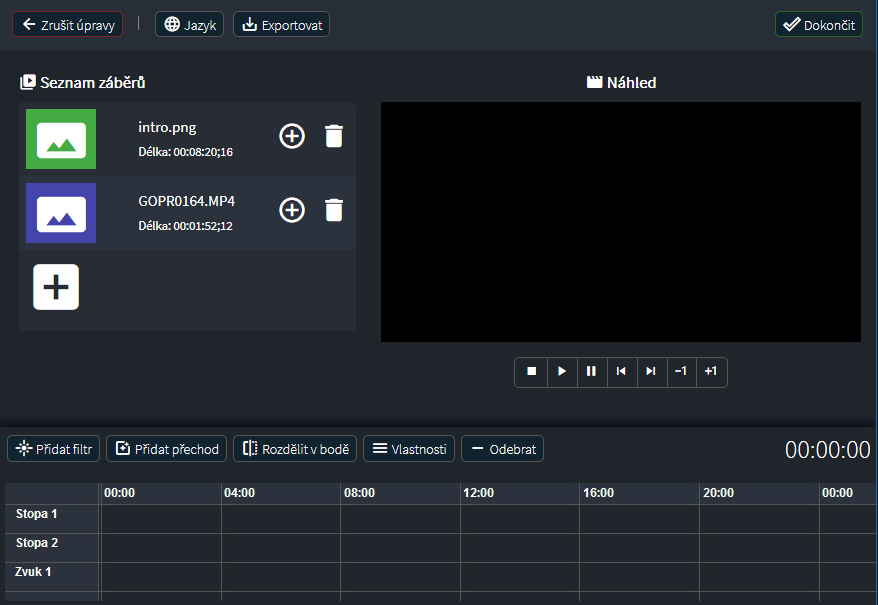
\includegraphics{obrazky-figures/mockup.png}
	}
	\caption{Prototyp uživatelského rozhraní.}\label{img:mockup}
\end{figure}

U~horního okraje obrazovky se nachází panel nástrojů pro globální akce nad projektem -- zrušit úpravy nebo renderovat projekt. Do budoucna zde bude možnost přepínat jazykovou mutaci a možnost exportu nebo výmazu dat.

Operace nad videi jsou členěny do 3 částí, tomu odpovídá a členění uživatelského rozhraní. V~levé části je seznam zdrojového materiálu (videí, obrázků, aj.), který je možné v~projektu použít. S~položkami seznamu se zdrojovým materiálem se pracuje přímo. Dostupné operace jsou zobrazeny po celou dobu. Pod poslední položkou se nachází tlačítko na přidání materiálu, případně je možné použít přetažení souboru do této oblasti. V~seznamu zdrojů je možné nahrávat obrázkové a video soubory. Podporované formáty video souborů jsou shodné s~formáty, které podporuje multimediální framework FFmpeg. Z~obrázkových souborů je podporován formát PNG a JPEG obrázek. Obrázek \ref{img:ucd-zdroj} zobrazuje diagram případů užití pro práci se zdrojovým materiálem.
% [Uživatel]-(Nahrát video nebo obrázek),
% [Uživatel]-(Odebrat video nebo obrázek),
% [Uživatel]-(Vložit video na konec časové osy),
% [Uživatel]-(Vložit obrázek na konec časové osy),
% (Vložit obrázek na konec časové osy)>(Nastavit dobu trvání),
\begin{figure}[h]
	\centering
	\scalebox{0.4}{
		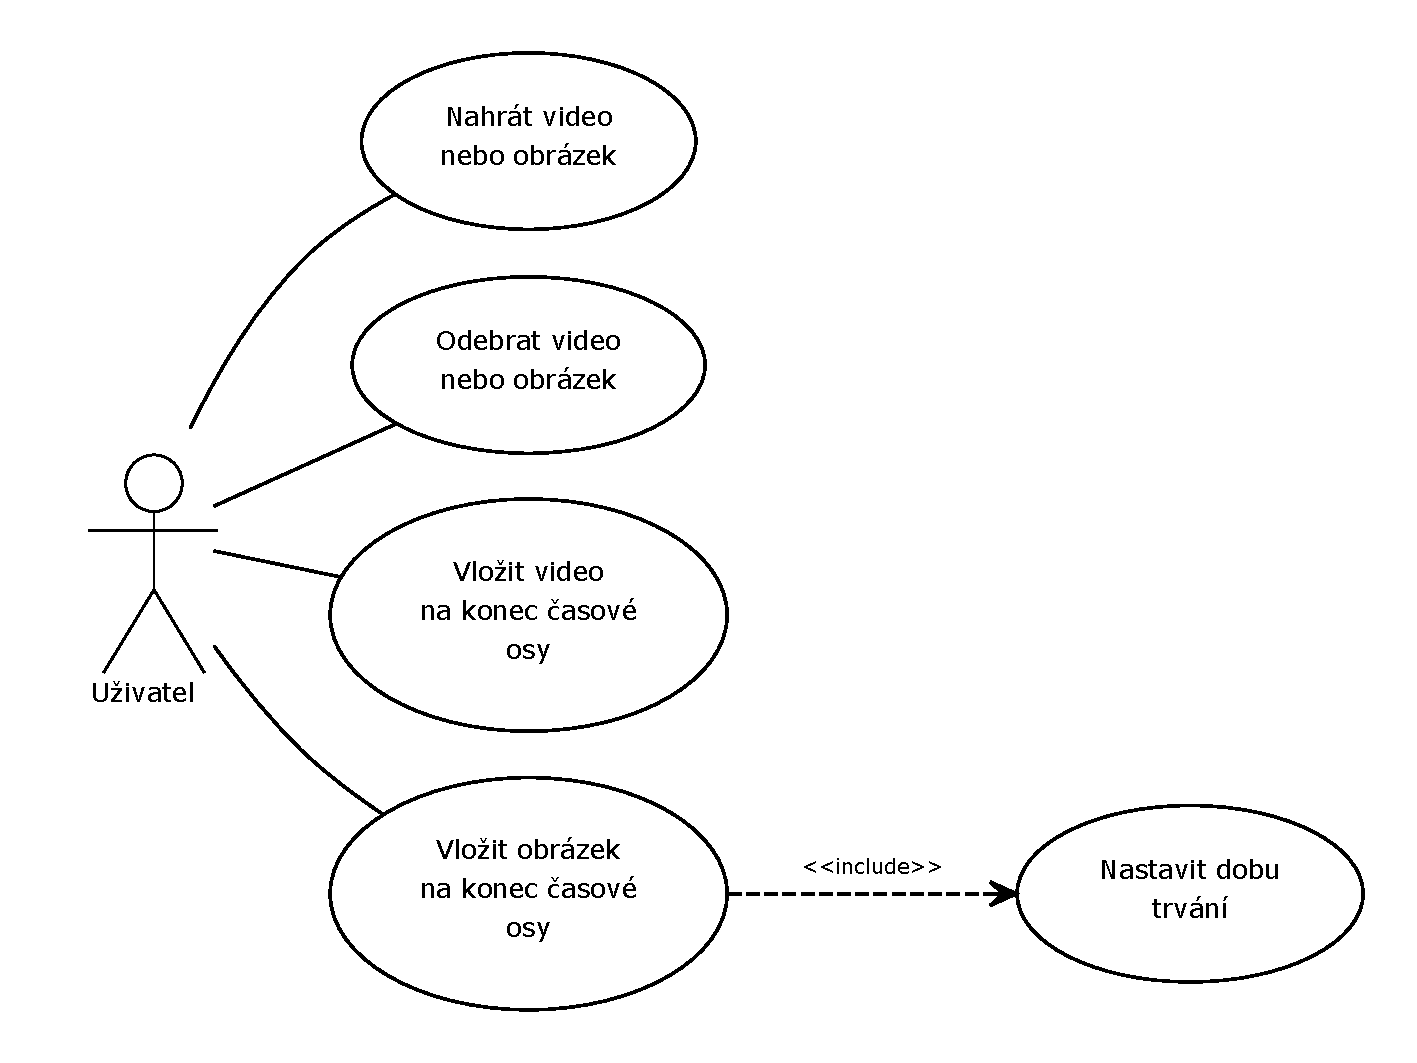
\includegraphics{obrazky-figures/ucd-zdroje.pdf}
	}
	\caption{Diagram případů užití pro práci se zdroji.}\label{img:ucd-zdroj}
\end{figure}

V~pravé polovině se nachází přehrávač předběžného náhledu výsledného videa. Přehrávač náhledu se ovládá tlačítky umístěnými přímo pod přehrávačem (přehrát, zastavit, skok na začátek nebo konec, skok na začátek nebo konec aktuální položky). Přehrávač přehrává pouze soubory umístěné na časové ose, nezobrazuje náhledy zdrojového materiálu. Aktuální pozici přehrávače udává ukazatel na časové ose. Přehrávání lze spustit původní rychlostí a pozastavit. K~manipulaci s~pozicí ve videu slouží skok na událost vpřed/vzad, který přesune ukazatel na nejbližší začátek nebo konec položky libovolné stopy, diagram případů užití zobrazuje obrázek \ref{img:ucd-prehravac}.
% [Uživatel]-(Spustit přehrávání),
% [Uživatel]-(Pozastavit přehrávání),
% [Uživatel]-(Skok na událost vpřed nebo vzad),
% [Uživatel]-(Další nebo předchozí snímek),
\begin{figure}[!h]
	\centering
	\scalebox{0.4}{
		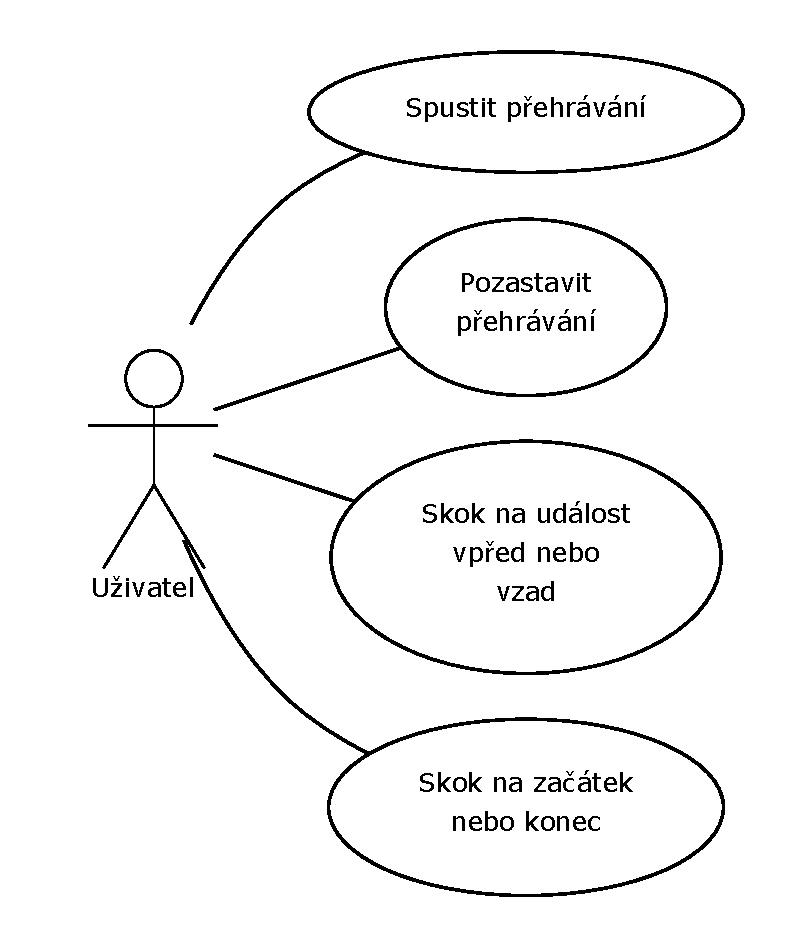
\includegraphics{obrazky-figures/ucd-prehravac.pdf}
	}
	\caption{Diagram případů užití pro práci s~přehrávačem náhledu.}\label{img:ucd-prehravac}
\end{figure}

Ve spodní části je časová osa se zvukovými a obrazovými stopami. Časová osa zobrazuje pod sebou stopy v~pořadí, v~jakém byly vytvořeny. Stopy se přidávají a odebírají podle potřeby. Pokud uživatel uchopí položku a přetáhne ji pod poslední video/audio stopu, vytvoří se nová. Původní návrh počítal se zobrazováním názvů stop a manuálním přidávání stop. Po testování jsem se rozhodl odstínit uživatele od stop a nabídnout mu pracovní plochu, kde může přesouvat položky i vedle sebe, bez nutnosti řešit stopy. Položky se na časovou osu přidávají ze seznamu materiálu tlačítkem plus u~materiálu. Posun položek na časové ose se provede uchopením prvku a přetažením na nové místo, přesun na jinou časovou se provádí přetažením na jinou osu stejného typu. Uchopením položky za okraj lze měnit začátek nebo konec. U~každé položky je náhledový obrázek a textové informace o~položce. S~vybranou položkou lze pracovat tlačítky na listě nástrojů u~horního okraje časové osy. V~aplikaci jsou dvě lišty nástrojů, globální akce a akce s~časovou osou. Pokud je na položku aplikován alespoň jeden filtr, zobrazí se v~jejím levém horním rohu \uv{nálepka} s~ikonou filtru. Časovou osu lze přibližovat a oddalovat tlačítky v~liště nástrojů časové osy. Pokud je časová osa přiblížena natolik, že není možné zobrazit všechny prvky časové osy, lze osu posouvat do stran uchopením prázdného místa na ose a přetažením osy do stran. V~novém projektu je k~dispozici prázdná zvuková a video stopa. Ukazatel aktuálního času lze uchopit a přesunout. V~čase ukazatele se bude přehrávat náhled videa a v~tomto čase lze provést střih videa, diagram případů užití -- obrázek \ref{img:ucd-osa}.
% [Uživatel]-(Přiblížit časovou osu),
% [Uživatel]-(Posunout časovou osu do stran),
% [Uživatel]-(Přidat nebo odebrat časovou osu),
% [Uživatel]-(Nastavit pozici ukazatele)
\begin{figure}[h]
	\centering
	\scalebox{0.4}{
		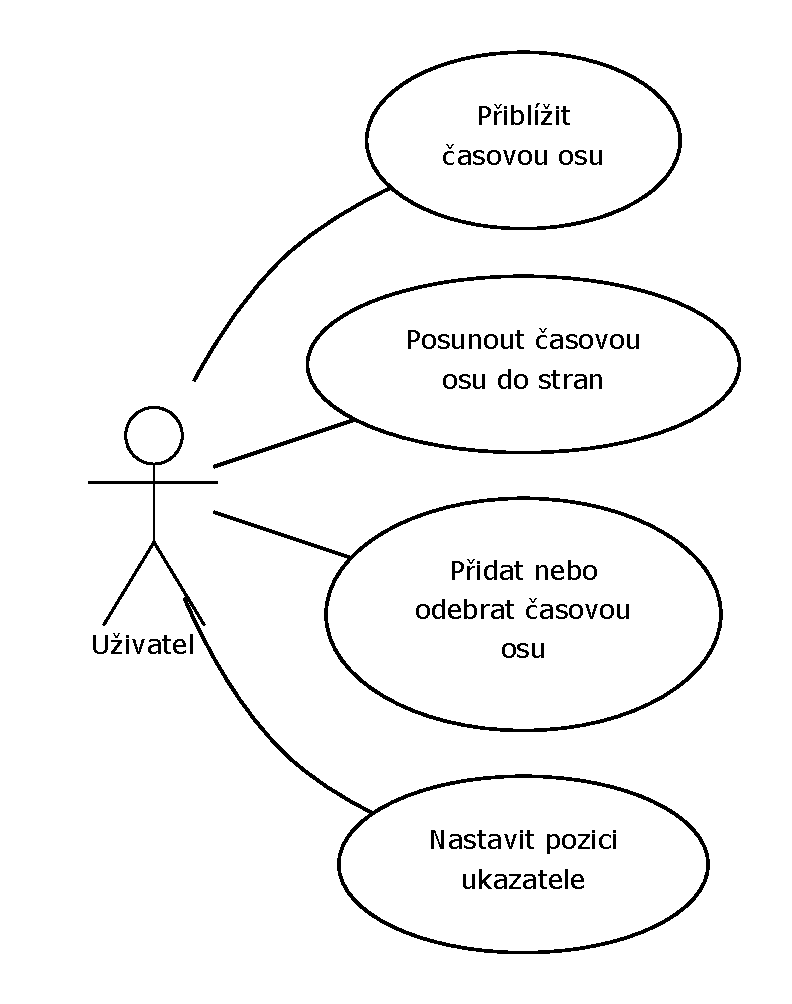
\includegraphics{obrazky-figures/ucd-osa.pdf}
	}
	\caption{Diagram případů užití pro práci s~časovou osou.}\label{img:ucd-osa}
\end{figure}

Po vybrání položky (videa nebo obrázku) na časové ose jsou k~dispozici v~panelu nástrojů časové osy následující akce. Položku lze smazat, okolní položky zůstávají, přechody se zruší. Lze přidat filtr obrazu (text, HTML překrytí, jas, kontrast, odstín, světlost, sytost, vyvážení bílé, otočit, velikost, poloha, ořezání, průhlednost, ostrost) nebo filtr zvuku (ztišit, zesílit/zeslabit). Přidat přechod prolnutí mezi 2 položkami, položky s~přechody se při přesouvání chovají jako celek. Dále lze zobrazit souhrnné vlastnosti. Následující úkony se neprovádí přes panel nástrojů --  a začátek nebo konec video souboru či délku obrázku lze změnit uchopením okraje položky a táhnutím na požadovanou pozici. Akce s~vybranou položkou zobrazuje diagram případů užití na obrázku \ref{img:ucd-polozky}.
% [Uživatel]-(Posunout na časové ose),
% [Uživatel]-(Přesunout na jinou časovou osu),
% [Uživatel]-(Vybrat pro práci),
% [Uživatel]-(Změnit začátek nebo konec ořezem),
% [Uživatel]-(Rozdělit v bodě na 2 části),
% (Vybrat pro práci)<(Odstranit z časové osy),
% (Vybrat pro práci)<(Přidat filtr),
% (Vybrat pro práci)<(Přidat přechod mezi 2 položkami),
% (Vybrat pro práci)<(Zobrazit vlastnosti),
\begin{figure}[!h]
	\centering
	\scalebox{0.4}{
		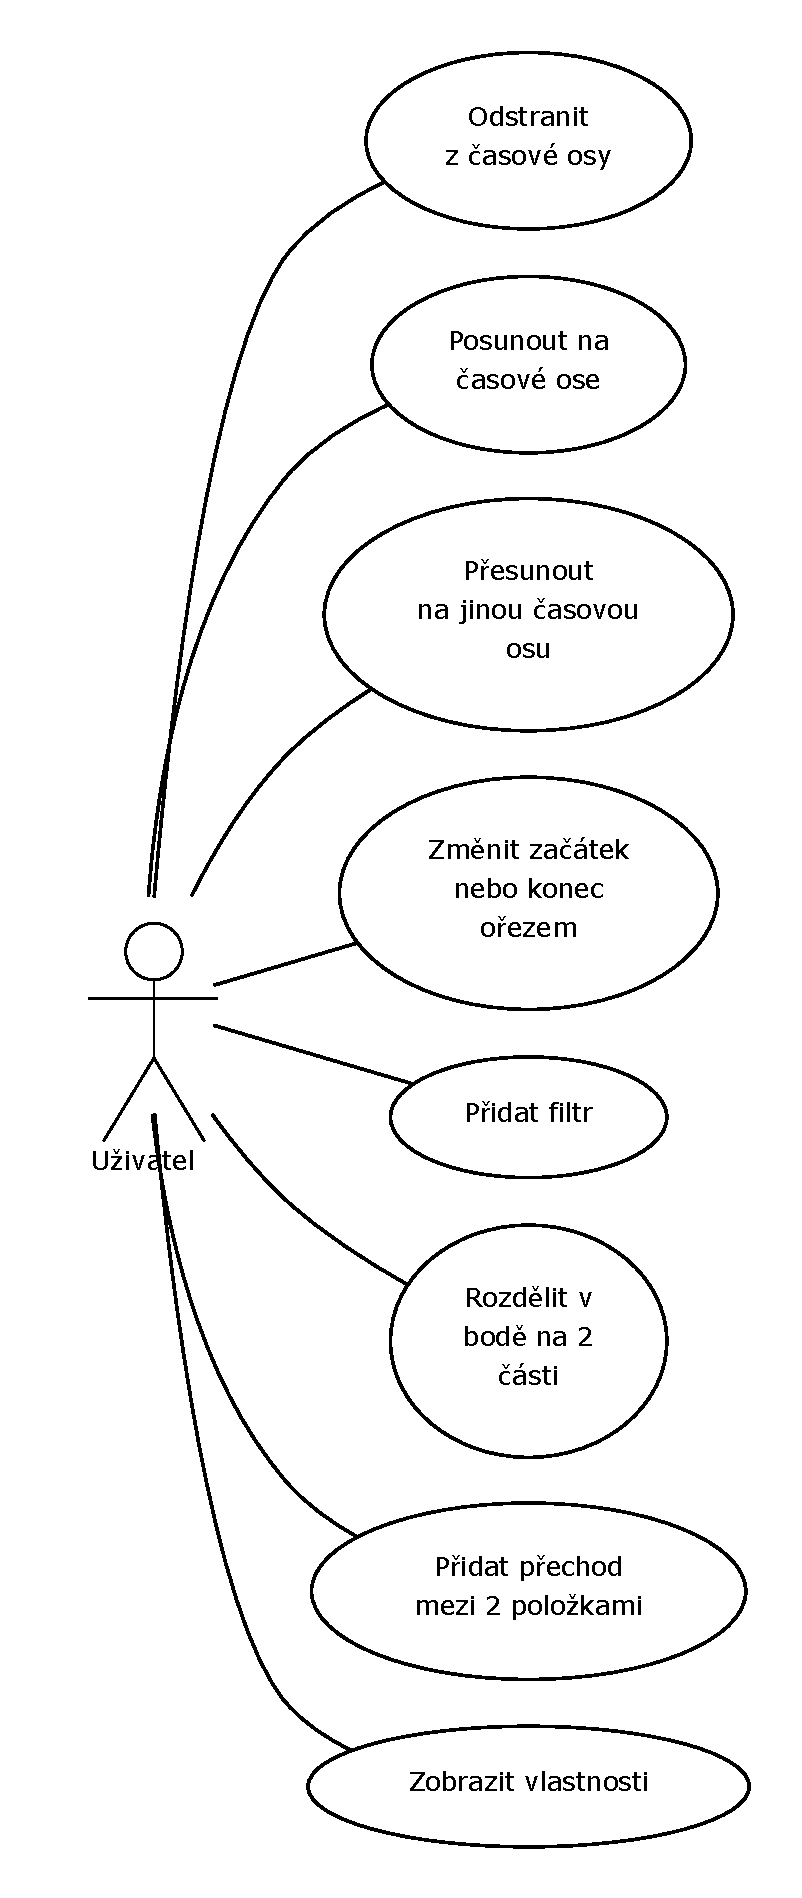
\includegraphics{obrazky-figures/ucd-polozky.pdf}
	}
	\caption{Diagram případů užití pro práci s~položkami časové osy.}\label{img:ucd-polozky}
\end{figure}

Pokud je potřeba upřesnit, jakou akci chce uživatel provést (výběr filtru), zobrazí se rozbalovací nabídka. Vyžaduje-li akce zadání hodnot, zobrazí se modální okno. Modální okna jsou využívána i pro zobrazení vlastností. Nápověda k~prvkům je řešena pomocí informačních bublin (někdy též tooltip).

Pokud má nový systém nahradit stávající proces zpracování videa, musí zvládat všechny kroky úprav videa. V~Tabulce \ref{tab:uc1} uvádím v~současnosti nejčastější případ užití, kdy je potřeba oříznout začátek a konec videa a před video vložit úvodní obrazovku s~podmínkami použití.

\begin{table}[h]
    \centering
    \begin{tabular}{|p{14cm}|}
        \hline
        Případ užití: Vložit intro, oříznout videozáznam\\ \hline
        \textbf{ID: UC1}\\ \hline
        \textbf{Účastníci:}\\
        Zaměstnanec FIT\\
        Systém\\ \hline
        \textbf{Vstupní podmínky:}\\
        1. Zaměstnanec má k~dispozici obrázek s~intro a video.\\
        2. Zaměstnanec otevřel internetové stránky s~editorem.\\ \hline
        \textbf{Tok událostí:}\\
        1. Případ užití začíná nahráním videa a obrázku intra.\\
        2. Uživatel vloží obrázek na časovou osu, v~dialogu nastaví délku zobrazení intra.\\
        3. Uživatel vloží video na časovou osu.\\
        4. Uživatel si přehraje náhled videa a v~místě plánovaného začátku a konce videa přehrávání pozastaví a provede rozdělení na 2 části.\\
        5. Uživatel zvolí část po plánovaném konci a odstraní ji.\\
        6. Uživatel zvolí část před plánovaným začátkem a odstraní ji. Ořezané video uchopí a přetáhne jej na časové ose hned za konec intra.\\
        7. Uživatel potvrdí změny a vyplní parametry výsledného videa.\\
        8. Systém generuje XML a nabízí jej ke stažení nebo zpracování na serveru.\\
        \hline
    \end{tabular}
    \caption{Textová specifikace případů užití pro nejčastější úpravy záznamů přednášek.}
    \label{tab:uc1}
\end{table}

\section{Návrh API}
Stejně jako uživatelské rozhraní i serverové rozhraní je potřeba navrhnout a otestovat. Při návrhu je třeba dbát pravidel architektury \textit{REST}. \textit{REST} definuje, jakým způsobem lze pracovat s~daty na serveru. K~práci se využívají 4 metody -- vytvoření dat (Create), získání požadovaných dat (Retrieve), změnu (Update) a smazání dat (Delete). Tato čtveřice bývá označování zkratkou CRUD\,\cite{rest}.

Nejprve jsem si ujasnil, jaké všechny operace bude API umožňovat. Jedná se o~následující operace: vytvořit nový projekt, získat stav existujícího projektu, nahrát soubor ze zařízení, vložit nahraný soubor na časovou osu, přidat filtr, odebrat filtr, přidat přechod, odebrat přechod, posunout položku, rozdělit položku na 2 části, odebrat položku z~časové osy, smazat nahraný soubor, renderovat projekt, případně smazat projekt.

Dalším krokem bylo identifikovat zdroje -- entity. Jednou z~entit bude beze sporu \textbf{projekt}, dále \textbf{soubor} a \textbf{položka časové osy}. Dalšími entitami jsem určil \textbf{přechod} a \textbf{filtr}. Operace je možné provádět jen nad zdroji, po identifikaci zdrojů je potřeba přiřadit operace ke zdrojům.

K~projektu jsem přiřadil: vytvořit nový projekt, získat stav existujícího projektu, renderovat projekt, smazat projekt. Nad souborem bude možné provádět: nahrát soubor ze zařízení, vložit nahraný soubor na časovou osu, smazat nahraný soubor. Položka časové osy bude umožňovat: posunout položku, rozdělit položku na 2 části, odebrat položku z~časové osy. Filtr bude možné přidat a odebrat, stejně tak přechod bude možné přidat a odebrat.

\textit{REST} ovšem rozlišuje 4 metody. Nyní je potřeba přiřadit operacím jednu z~následujících metod: POST (Create), GET (Retrieve), PUT (Update), DELETE (Delete). Nové prostředky vytváříme při vytváření nového projektu, nahrávání souboru ze zařízení, přidání filtru a přechodu, pro tyto operace jsem zvolil metodu POST. Získávání stavu projektu je jednoznačně metoda GET. Pro rušení prostředků slouží metoda DELETE -- odebrání filtru, odebrání přechodu, odebrání položky z~časové osy, smazání nahraného souboru, smazání projektu. Na zbývající operace jsem použil metodu PUT -- vložit nahraný soubor na časovou osu, posunout položku, rozdělit položku na 2 části.

I~ideálním případě nevzniknou kolize a každý zdroj bude mít přiřazenou maximálně jednu operaci k~jedné HTTP metodě. V~mém případě má zdroj \textbf{položka na časové ose} dvě metody PUT -- posunout položku, rozdělit položku na 2 části. V~této chvíli je potřeba operace dále rozlišit, přesun identifikuji jako \texttt{move} a rozdělení položek jako \texttt{split}.

Aby nemohlo dojít ke kolizi mezi URL určených pro webové stránky a pro API, mají veškeré požadavky na API prefix \texttt{api}. Do budoucna to umožní například verzovat API. Výsledný návrh API uvádím v~následujícím seznamu:
\begin{itemize}
\item project
\begin{itemize}
\item POST: \texttt{/project}
\item GET: \texttt{/project/\{projectID\}}
\item DELETE: \texttt{/project/\{projectID\}}
\item PUT: \texttt{/project/\{projectID\}}
\end{itemize}
\item file
\begin{itemize}
\item POST: \texttt{/project/\{projectID\}/file}
\item DELTE: \texttt{/project/\{projectID\}/file/\{fileID\}}
\item PUT: \texttt{/project/\{projectID\}/file/\{fileID\}}
\end{itemize}
\item filter
\begin{itemize}
\item POST: \texttt{/project/\{projectID\}/filter}
\item DELETE: \texttt{/project/\{projectID\}/filter}
\end{itemize}
\item transition
\begin{itemize}
\item POST: \texttt{/project/\{projectID\}/transition}
\item DELETE: \texttt{/project/\{projectID\}/transition}
\end{itemize}
\item item
\begin{itemize}
\item DELETE: \texttt{/project/\{projectID\}/item}
\item PUT: \texttt{/project/\{projectID\}/item/move}
\item PUT: \texttt{/project/\{projectID\}/item/split}
\end{itemize}
\end{itemize}

Požadavek na \textit{REST} API musí být úplný, \textit{REST} API je bezstavové. Například požadavek DELETE \texttt{/project/\{projectID\}} je úplný, serveru říkáme, že má smazat projekt a zároveň i uvádíme identifikátor projektu. U~některých požadavků je ale potřeba blíže specifikovat parametry požadavku. Například u~požadavku POST: \texttt{/project/\{projectID\}/filter} nevíme, jaký filtr se má aplikovat a ani nevíme, na jakou položku. Vyjma metody GET mohou mít požadavky tělo s~parametry. Parametry mohou být předány v~libovolném formátu, v~projektu používám \textit{application/json} a pro nahrávání souboru \textit{multipart/form-data}. Přechozí požadavek je upřesněn parametry \texttt{track}, \texttt{item}, \texttt{filter} a \texttt{params} (parametry filtru). Kompletní specifikace navrženého API se nachází v~dokumentaci API. API jsem zdokumentoval dle specifikace \textit{OpenAPI 3.0}\,\footnote{OpenAPI 3.0 -- komunitní specifikace pro popis REST API, \url{https://www.openapis.org/}.} pomocí online nástroje \textit{Swagger Editor}\,\footnote{Swagger Editor -- open source online editor pro dokumentování API, \url{https://editor.swagger.io/}.}.

\chapter{Práce s multimédii}
\section{MLT framework}
Jedná se o~sadu nástrojů s~otevřeným zdrojovým kódem s~licencí LGPL-2.1, která byla původně vytvořena pro televizní vysílání. Poskytuje nástroje pro streamování, video editory, multimediální přehrávače, konvertory a další typy multimediálních aplikací. Framework MLT umožňuje vytvářet, spravovat a přehrávat audio nebo video projekty s~více stopami. Je používán jako základní komponenta v~nelineárních video editorech. Využití nalezne i mimo klasické desktopové video editory, může být použit jako součást většího systému nezávisle na použitém programovacím jazyce.

Framework lze používat prostřednictvím programu \texttt{melt} v~příkazovém řádku nebo prostřednictvím MLT API knihovny v~jazyce C. Pro napojení API na jiné programovací jazyky je nutné použít \textit{SWIG}\,\footnote{SWIG -- nástroj pro vývoj softwaru umožňující propojit program napsaný v~jazyce C/C++ s~jiným jazykem, \url{http://swig.org/}.}, nástroj, který překládá volání funkcí API na volání funkcí v~C++. V~C++ funkcích se následně volají funkce programu MLT v~jazyce C. Druhou možností je provádět serializaci/deserializaci dat vlastnoručně a s~MLT komunikovat prostřednictvím formátu XML. Vnitřní struktura, kterou MLT API vytváří je XML formátu blízká. V~této práci se zabývám využitím MLT XML.

\subsection{Zprovoznění}
Framework nemá žádné jiné závislosti, než standard C99 a knihovny standardu POSIX. Zprovoznění tak zahrnuje nainstalování programu \texttt{melt} (v~případě Ubuntu z~repozitáře) a nainstalovaní programů a kodeků pro práci s~multimédii.
\begin{lstlisting}[style=bash]
$ sudo apt install melt
$ sudo apt install ladspa-sdk ffmpeg
$ sudo apt install vlc #Volitelne, pro prehrani vystupu
\end{lstlisting}

\subsection{Základní příkazy}
Jednoduché úkony lze provádět volbou parametrů při spuštění programu. Pro složitější projekty bude potřeba použít serializaci dat a formát XML. Melt umí soubory XML načítat i generovat.
\begin{lstlisting}[style=bash]
#Prehrani na obrazovce
$ melt VIDEO0004.mp4 -consumer sdl
#Predpis pro vytvoreni sedotonoveho videa serializovany v~XML souboru
$ melt VIDEO0004.mp4 -filter greyscale -consumer xml > task.mlt 
#Renderovani souboru output.avi na zaklade XML souboru
$ melt task.mlt -consumer avformat:output.avi acodec=libmp3lame vcodec=libx264
\end{lstlisting}
\subsection{Používání formátu XML}
Nejprve je nutné uvést seznam vstupních mediálních souborů. Vstupný soubor je označen jako \texttt{producer}. U~vstupu se v~\texttt{property} uvádí hodnota \texttt{resource}, s~cestou k~souboru. Tento jednoduchý soubor po spuštění přehraje celý soubor VIDEO001.mp4. Toto XML může být užitečné, pokud chceme soubor pouze zkonvertovat do jiného formátu.
\begin{lstlisting}[style=xml]
<?xml version="1.0"?>
<mlt>
  <producer id="producer0">
    <property name="resource">/home/vladan/VIDEO0001.mp4</property>
  </producer>
</mlt>
\end{lstlisting}
Obvykle potřebujeme pracovat s~více soubory. K~tomuto účelu slouží \texttt{playlist}. Stanovíme vstupy (\texttt{producer}) s~unikátním \texttt{id}. V~tuto chvíli by se přehrál pouze poslední soubor, který uvedeme, neboť framework MLT přehraje vždy poslední element uvnitř kořenového elementu \texttt{<mlt>} . Definujeme \texttt{playlist} obsahující položky \texttt{entry}. Vstupní soubory jsou na výstup řazeny ve stejném pořadí v~jakém jsou uvedeny v~playlistu. U~položky playlistu můžeme uvést čas (od/do) pokud chceme vložit část vstupního souboru. Časové údaje lze zadávat buď jako počet snímků nebo jako čas ve formátu \texttt{00:00:00,000}, kde první dvojice číslic jsou hodiny a poslední tři číslice udávají milisekundy. Omezení se ignoruje, pokud uvedeme větší číslo, než je počet snímků či délka souboru. Vkládáme-li obrázek, pak hodnota \texttt{out} udá délku zobrazení obrázku. S~tímto XML zvládneme sestříhat více souborů do jednoho, vystřihnout určitou pasáž, vložit intro a outro.
\begin{lstlisting}[style=xml]
<?xml version="1.0"?>
<mlt>
  <producer id="producer0">
    <property name="resource">/home/vladan/VIDEO0004.mp4</property>
  </producer>
  <producer id="producer1">
    <property name="resource">/home/vladan/VIDEO0001.mp4</property>
  </producer>
  <producer id="producer2">
    <property name="resource">/home/vladan/lego1.png</property>
  </producer>

  <playlist id="playlist0">
    <entry producer="producer2" in="0" out="50"/>
    <entry producer="producer1" in="0" out="999"/>
    <entry producer="producer0" in="0" out="100"/>
  </playlist>
</mlt>
\end{lstlisting}
Chceme-li na video aplikovat filtry, musíme vytvořit element \texttt{tractor} obsahující \texttt{multitrack} se seznamem tracků (playlistů). V~tractoru definujeme filtry. Filtry aplikujeme na \texttt{track} (playlist). Pokud budeme chtít vzít vstupní video, aplikovat na něj černobílý filtr, musíme vytvořit \texttt{playlist} s~jedním zdrojem a \texttt{tractor} s~jedním playlistem (track).
\begin{lstlisting}[style=xml]
<?xml version="1.0"?>
<mlt>
  <producer id="producer0">
    <property name="resource">/home/vladan/VIDEO0002.mp4</property>
  </producer>
  <tractor id="tractor0">
    <multitrack>
      <playlist id="playlist0">
        <entry producer="producer0"/>
      </playlist>
    </multitrack>
    <filter mlt_service="greyscale" track="0"/>
  </tractor>
</mlt>
\end{lstlisting}
Pokud potřebujeme aplikovat filtr na část videa, musíme vytvořit dva playlisty -- jeden pro část na kterou bude aplikován filtr a druhý playlist pro část bez filtru. Pro synchronizaci playlistů použijeme \texttt{blank}, v~jednu chvíli se může zobrazovat pouze jeden z~playlistů, přednost má ten později definovaný. V~následujícím případě se v~playlist1 prvních 100 snímků přehrává VIDEO0002, v~playlist2 je po tuto dobu nastaven stav \texttt{blank}. Pokud chceme zobrazovat statickou překryvnou vrstvu, můžeme využít filtru \texttt{watermark}. Pokud je filtr přizpůsobitelný parametry, uvedou se uvnitř elementu \texttt{filter} stejným způsobem, jako se uvádí parametry u~elementů \texttt{producer}.
\begin{lstlisting}[style=xml]
<?xml version="1.0"?>
<mlt>
  <producer id="producer0">
    <property name="resource">/home/vladan/VIDEO0002.mp4</property>
  </producer>
  <tractor id="tractor0">
    <multitrack>
      <playlist id="playlist0">
        <entry producer="producer0" in="0" out="99"/>
        <blank length="50"/>
        <entry producer="producer0" in="150"/>
      </playlist>
      <playlist id="playlist1">
        <blank length="100"/>
        <entry producer="producer0" in="100" out="149"/>
      </playlist>
    </multitrack>
    <filter mlt_service="watermark" track="0">
      <property name="resource">transparent.png</property>
    </filter>
    <filter mlt_service="greyscale" track="1"/>
  </tractor>
</mlt>
\end{lstlisting}
Více stop (\texttt{track}) může být přehráváno současně pouze použijeme-li filtr nebo přechod. Přechody (\texttt{transition}) se aplikují stejně jako filtry uvnitř tractoru. U~přechodu nastavíme snímek náběhu a dokončení přechodu (\texttt{in} a \texttt{out}) a dále specifikujeme typ přechodu (\texttt{mlt\_service}) dle \url{https://www.mltframework.org/plugins/PluginsTransitions/}, počáteční stopu přechodu (\texttt{a\_track}) a cílovou stopu přechodu (\texttt{b\_track}). Tímto způsobem můžeme vytvořit intro nebo outro s~přechody, či prolínání jednotlivých video souborů. Obě stopy by se měly překrývat pouze po dobu přechodu. Pokud by například přechod skončil dříve, než by začala druhá stopa, docházelo by ke krátkodobému probliknutí první stopy.
\begin{lstlisting}[style=xml]
<mlt>
  <producer id="producer0">
    <property name="resource">lego1.png</property>
  </producer>
  <producer id="producer1">
    <property name="resource">VIDEO0001.mp4</property>
  </producer>
  <tractor id="tractor0">
    <multitrack id="multitrack0">
      <playlist id="playlist0">
        <entry producer="producer0" in="0" out="74"/>
      </playlist>
      <playlist id="playlist1">
        <blank length="50"/>
        <entry producer="producer1"/>
      </playlist>
    </multitrack>
    <transition mlt_service="luma" in="50" out="74" a_track="0" b_track="1"/>
  </tractor>
</mlt>
\end{lstlisting}

S~pomocí těchto konstrukcí jsme schopni nadefinovat nejčastější operace, které se při zpracovávání přednášek provádí.

\section{Práce s videi v prohlížeči}
S~příchodem HTML5 prvků \texttt{<video>} a \texttt{<audio>} a jejich JavaScriptového API vzniká možnost práce s~multimédií na webu. Práci s~multimediálními prvky implementovali od roku 2010 všechny moderní prohlížeče. Za moderní desktopové prohlížeče považuji program Google Chrome, Safari, Mozilla Firefox, Opera, Microsoft Edge. Prohlížeč Internet Explorer má sice dle serveru StatCounter 5.48\% zastoupení, což jej řadí mezi Microsoft Edge a Operu\,\cite{statcounter}, avšak i Microsoft jej v~únoru označil za \uv{řešení pro kompatibilitu}, nikoliv webový prohlížeč\,\cite{internetExplorer}. Po představení prohlížeče Microsoft Edge získává Internet Explorer bezpečnostní záplaty, ale neprobíhá implementace nových webových standardů. Při vývoji nových projektů by tedy nekompatibilita s~Internet Explorer neměla být brána v~potaz. Následující kapitoly čerpají z~knihy \textit{HTML5 - audio a video: kompletní průvodce}\,\cite{HTML5multimedia} a z~komunitního projektu MDN Web Docs\,\footnote{MDN Web Docs -- portál s~webovou dokumentací provozovaný společností Mozilla, \url{https://developer.mozilla.org/}.}.

\subsection{Kódování mediálních zdrojů}
Veškerá data v~počítači je potřeba kódovat. Na vyšší úrovni pohlížíme na kódování jako na formát dat. Formáty kódování audia  jsou například MP3, AAC, Vorbis, FLAC a formáty kódování videa například MPEG-2, MPEG-4 , H.264, HEVC, Theora, VP9, AV1.  Z~pohledu uživatele se liší zejména licencí pro použití a způsobem komprese dat. Multimediální soubory mohou obsahovat více video a audio stop, titulky či jiná podpůrná data, proto se multimediální soubory vždy obalují do multimediálních kontejnerů, jako například AVI, MP4, FLV, RealMedia, Matroška. Výběr formátu videa tak typicky zahrnuje výběr multimediálního kontejneru, formátu kódování videa a formátu kódování audia. Kodek je zařízení nebo počítačový program, který dokáže převádět zakódovaná data do jiné podoby, v~případě webových aplikací je kodekem internetový prohlížeč. V~době, kdy organizace W3C\,\footnote{World Wide Web Consortium (W3C) -- mezinárodní sdružení vytvářející webové standardy, \url{https://www.w3.org/}.} vytvářela specifikaci pro HTML5 prvky \texttt{<video>} a \texttt{<audio>}, byla snaha standardizovat formát, který by byl podporován ve všech prohlížečích neúspěšná kvůli požadavku na royalty free licenci\,\cite{HTML5multimedia}. Od té doby se nejvíce rozšířil formát MP4 H.264, který ovšem odmítá Mozilla a Theora, který odmítá Apple. Pokud se podíváme dnes na srovnání podporovaných kodeků, tabulka \ref{tab:codecs}, zjistíme, že situace není jednoduchá.
\begin{table}[h]
    \centering
    \begin{tabular}{|l|l|l||l|l|l|l|l|}
    \hline
    Kontejner   & Video & Audio & Chrome & Firefox & Edge & Opera & Safari \\
    \hline
    WebM        & VP8   & Vorbis &ano & ano & s~2 rozšířeními & ano & ne* \\
    WebM        & VP9   & Opus & ano & ano & rozšíření, HW dekodér & ano & ne \\
    WebM        & AV1   & Vorbis & ano & ano & s~beta rozšířením & ano & ne \\
    WebM        & AV1   & Opus & ano & ano & s~beta rozšířením & ano & ne \\
    Ogg         & Theora & Vorbis & ano & ano & s~rozšířením & ano & ne \\
    MP4         & H.264 & MP3 & ano*** & ano** & ano & ano & ano \\
    MP4         & H.264 & AAC & ano*** & ano** & ano & ano & ano \\
    \hline
    \end{tabular}
    \caption{Přehled široce podporovaných formátů videa internetovými prohlížeči.}
    \label{tab:codecs}
\end{table}\\
* Safari vyžaduje pro VP8 program Perian\,\footnote{Perian -- program pro MacOS rozšiřující podporu QuickTime o~další formáty (vývoj ukončen), \url{https://www.perian.org/}.}.\\
** Mozilla Firefox pro Linux vyžaduje pro H.264 program GStreamer\,\footnote{GStreamer -- otevřený multiplatformní multimediální framework, \url{https://gstreamer.freedesktop.org/}.} nebo FFmpeg.\\
*** Google Chrome H.264 podporuje, ale Chromium vyžaduje FFmpeg.
\medskip

Pokud bychom chtěli použít pouze jeden formát, můžeme zvolit H.264 video s~AAC audiem uvnitř MP4 nebo VP8 video s~Vorbis audiem uvnitř WebM. V~prvním případě budou muset uživatelé prohlížeče Firefox na Linuxových systémech a uživatelé prohlížeče Chromium nainstalovat program FFmpeg, v~druhém případě budou muset uživatelé Safari nainstalovat program Perian a uživatelé Microsoft Edge Rozšíření pro webová média a Rozšíření pro video VP9.

Chceme-li mít jistotu, že uživatel video přehraje, pak musíme zvolit formáty dva -- H.264 s~MP3/AAC uvnitř MP4 pro uživatele Safari a Edge a pro ostatní uživatele variantu Theora s~Vorbis uvnitř Ogg.

\subsection{Použití prvku video}
Prvek \texttt{<video>} přinesla specifikace HTML5 a umožňuje přehrávat video na webové stránce v~režii prohlížeče. Pokud nespecifikujeme jinak, prohlížeč zajistí načtení zdroje a vykreslení ovládacích prvků. S~videem můžeme pracovat skrze atributy a HTMLMediaElement API. Prvek je podporován všemi rozšířenými prohlížeči s~výjimkou Opera Mini (kvůli spořiči přenesených dat).

Video prvek má celkem 6 atributů. Atributy \texttt{autoplay}, \texttt{loop} a \texttt{controls} mohou nabývat booleovských hodnot, a proto jejich uvedení znamená logickou 1, pokud atributy neuvedeme, jsou atributy s~hodnotou logické 0. Pro potřeby náhledu videa atribut \texttt{autoplay} nepoužijeme, video budeme přehrávat skrze API metody \texttt{play}, \texttt{loop} rovněž není žádoucí, video by se přehrávalo ve smyčce, při neuvedení se přehrávání na konci zastaví. Atribut \texttt{controls} zobrazí ovládací prvky, což je nežádoucí, použijeme vlastní ovládací prvky. Atribut \texttt{preload} navrhuje prohlížeči, kolik dat se má načíst ze zdroje, dostupné hodnoty jsou \uv{none}, \uv{metadata} a \uv{auto}. Hodnota \uv{none} nenačte nic, \uv{metadata} zajistí načtení délky videa a prvního snímku, \uv{auto} nechá volbu na prohlížeči. V~případě editoru postačuje výchozí hodnota \uv{auto}. Atribut \texttt{poster} slouží k~nahrazení prvního snímku zástupným obrázkem, v~projektu není potřebný. Praktické jsou elementy \texttt{width} a \texttt{height}, udávají šířku a výšku videa. Rozměry jsou chápány jako maximální možné, pokud je rozměr videa větší, zmenší se ve výchozím nastavení se zachováním poměru stran. Zarovnání videa v~boxu určuje CSS vlastnost \texttt{object-position} s~dvojicí hodnot pro vodorovnou a svislou pozici. Jak se má měnit měřítko obsahu videa vlastnost \texttt{object-fit} s~hodnotami \uv{fill}, \uv{contain} a \uv{cover}.

Zdroj videa lze nastavit dvěma způsoby. Atributem \texttt{src} nebo vnořenými prvky \texttt{<source>}. Vnořené prvky \texttt{<source>} poskytují více možností skrze vlastní atributy. Zdrojů můžeme uvést více s~různými formáty -- atribut \texttt{type} (MIME typ mediální zdroje) nebo \texttt{media} (mediální zdroj pro konkrétní typ zařízení). Prohlížeč sám vybere pro něj nejlepší zdroj. Pokud měníme zdroje dodatečně, musíme po změně zavolat metodu \texttt{load}, která provede inicializaci video prvku. Druhou možností je uvést zdroj v~atributu \text{src} prvku \text{<video>}. Takto je možné nastavit jen jeden zdroj současně, a proto si musíme kompatibilitu formátu sami skrze metodu \texttt{canPlayType} nebo knihovny Modernizer\,\footnote{Modernizer -- sada nástrojů pro testování funkcí prohlížeče, \url{https://modernizr.com/}.}. Druhá metoda je vhodná pokud používáme jeden zdroj.

\subsection{Použití prvku audio}
Prvek pro přehrávání audia v~prohlížeči je možné rovněž upravovat pomocí HTMLMediaElement API a pomocí atributů. Prvek \texttt{<audio>} narozdíl od videa nemá atributy \texttt{poster}, \texttt{width}, \texttt{height}, protože jsou v~prohlížeči vykresleny pouze ovládací prvky bez vizualizace audia. Audio prvek lze využít pro zvukové stopy. Nastavení a význam hodnot atributů je stejný jako u~prvku \texttt{<video>}.

\subsection{Ovládání videa}
Přehrávání videa lze ovládat pomocí JavaScriptu skrze HTMLMediaElement API. Stejné API používají i prvky \texttt{<audio>}, lze pro ně použít stejný postup. Základními metodami pro přehrávání jsou \texttt{play} a \texttt{pause}. Přehrávání videa se na konci zastaví (pokud není nastaven atribut \texttt{loop}). Pokud po dokončení přehrávání zavoláme znovu metodu \texttt{play}, přehrávání se spustí od začátku videa.

Pro skok na konkrétní pozici slouží atribut \texttt{currentTime}. Atribut je určen pro čtení (získání aktuálního času) i pro zápis (skok na pozici). Celkovou délku zjistíme přečtením atributu \texttt{duration}. Délku musíme zjišťovat až po získání metadat -- odpálení události \texttt{loadedmetadata}.

Další užitečnou událostí je \texttt{timeupdate}, která se volá v~intervalech 15 ms až 250 ms (Mozilla Firefox 100-250 ms) po čas přehrávání a umožňuje průběžně efektivně pracovat s~atributem \texttt{currentTime} a například zobrazovat aktuální pozici přehrávání.

Použití událostí a metod pro jednoduchý přehrávač videa řízený JavaScriptem ukazuje obrázek \ref{img:html-control}.

\begin{figure}[h]
	\centering
	\scalebox{0.7}{
		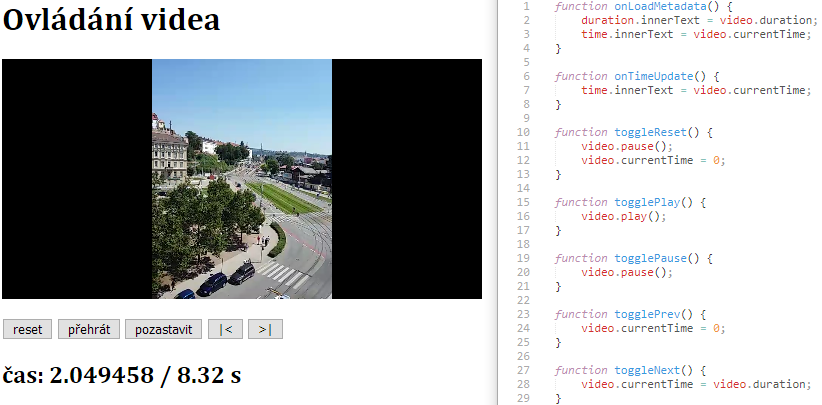
\includegraphics{obrazky-figures/html-control.png}
	}
	\caption{Jednoduchý přehrávač videa demonstrující využití HTMLMediaElement API.}\label{img:html-control}
\end{figure}

\subsection{Posloupnost videí}
Při dosažení konce média je odpálena událost \texttt{ended}. Této události lze využít pro vytváření posloupnosti videí. Plocha s~náhledem je tvořena dvojicí videí. Na popředí je aktuálně přehrávající se videa a na pozadí je skryté druhé video, které se s~předstihem nastaví na nový zdroj, počáteční pozici a načtou se metadata. Jakmile přehrávání videa v~popředí skončí a je odpálena událost \texttt{ended}, dojde k~prohození videa v~popředí s~videem v~pozadí a spustí se nové video v~popředí. Přístup dvou scén, kdy jedna je viditelná a druhá se připravuje, je inspirován programem OBS Studio\,\footnote{OBS Studio -- open source software pro nahrávání a streamování videí, \url{https://obsproject.com/}.}, který slouží na nahrávání a streamování videí. Ve webovém prohlížeči určuje pořadí objektů CSS vlastnost \texttt{z-index}. Hodnotou je celé číslo, objekty s~vyšší hodnotou překryjí objekty s~nižší hodnotou. Prvky se musejí překrývat, to lze zajistit absolutním pozicování uvnitř kontejneru. Následující kód obsahuje funkci pro přehození video souborů a pro resetování přehrávače do původního stavu.
\begin{lstlisting}[style=JavaScript]
let videoMain = video1;
function videoSwap() {
    videoMain = video2;
    video1.style.zIndex = 1;
    video2.style.zIndex = 2;
    togglePlay();
}

function toggleReset() {
    videoMain.pause();
    video1.currentTime = 0;
    video2.currentTime = 0;
    video1.style.zIndex = 2;
    video2.style.zIndex = 1;
    videoMain = video1;
}
\end{lstlisting}
Pro posloupnost více videí je zapotřebí \uv{podavač} videí, který přehrávači předá další klip.

\subsection{Přechod mezi videi}
Při stříhání videí se může hodit efekt prolnutí mezi 2 klipy. Při tomto přechodu se určitý čas před koncem přehrávaného videa začne přehrávat i video následující a současné video se postupně zprůhlední. Průhlednost elementů lze nastavit CSS stylem \texttt{opacity}, přičemž hodnota 1 značí neprůhledný objekt a hodnota 0 zcela průhledný objekt. Samotné prolnutí (zvyšování průhlednosti) lze provést CSS animacemi nebo snižováním hodnoty \texttt{opacity} s~každým odpálením události \texttt{timeupdate}. Použití animací sice vytvoří plynulý efekt, ale nastává problém při pozastavení a obnovení videa v~místě přechodu, neboť by animace musela být pozastavena, aktuální stav uložen a posléze vytvořena nová animace pro zbývající úsek. Řešení pomocí \texttt{timeupdate} poskytuje pro náhled dostatečnou kvalitu a provést pozastavení či skok je v~tomto případě snadné. Pokud chceme aplikovat prolnutí, stačí nastavit délku přechodu a poté zaregistrovat následující funkci pro obsluhu události \texttt{timeupdate}.
\begin{lstlisting}[style=JavaScript]
videoMain.addEventListener('timeupdate', transitionLuma, false);
function transitionLuma() {
    const timeToEnd = videoMain.duration - videoMain.currentTime;
    if (timeToEnd <= transitionDuration) {
        videoMain.style.opacity = (timeToEnd / transitionDuration);
        if (!transition) {
            videoBack.play();
            transition = true;
        }
    }
}
\end{lstlisting}
Na každou událost lze zaregistrovat více obslužných funkcí, po skončení přechodu je nutné obsluhu funkcí \texttt{transitionLuma} odregistrovat. Pokud je zbývající čas menší nebo roven délce přechodu, nastaví se \texttt{opacity} na hodnotu rovnou podílu zbývajícího času s~délkou přechodu (klesá rovnoměrně od 1 k~0). Ve webovém prohlížeči lze sestrojit i jiné přechody s~odsunutím, zvětšováním, postupným odkrýváním, ale tyto filtry nejsou pro tvorbu přednášek vhodné a proto je není potřeba implementovat.

Stejnou technikou se sestrojí roztmívání a zatmívání obrazu (přechod z~černé / do černé), pouze bude druhá scéna až za podkladovou černou vrstvou (\texttt{z-index se zápornou hodnotou}).

\subsection{Filtry}
Pokud potřebujeme aplikovat filtr obrazu, nabízí se dvě možnosti -- řešení pomocí CSS filtrů a řešení pomocí vykreslování do Canvas. Obě varianty mají své přednosti, CSS najde uplatnění u~jednoduchých filtrů, vykreslování do Canvas nám dá absolutní kontrolu nad výsledným videem.

\subsubsection{Obrazové filtry pomocí CSS}
HTML5 obsahuje pracovní návrh CSS vlastnosti \texttt{filter}. Vlastnost aplikuje grafické efekty na libovolné objekty, včetně obrázků a video elementů. CSS vlastnost má několik definovaných filtrů a možnost odkazovat na SVG filtry. Ačkoliv se jedná o~pracovní návrh, CSS filtry jsou podporovány všemi rozšířenými prohlížeči (Internet Explorer je nepodporuje)\,\cite{MDNfilter}. Microsoft Edge podporuje předdefinované filtry, ale kvůli chybě nepodporuje odkazování na SVG filtry. Největší předností CSS filtrů je způsob aplikování na video. Filtr je uložen v~CSS třídě, případně lze přiřadit přímo k~elementu. U~\texttt{<video>} elementu stačí nastavit třídu filtru a filtr se aplikuje, vykreslování zajistí prohlížeč. Jaké předdefinované filtry vlastnost \text{filter} nabízí, ukazuje tabulka \ref{tab:filters}.
\begin{table}[h]
    \centering
    \begin{tabular}{|l|l|l|l|l|l|l|l|}
    \hline
    Funkce filtru   & Výchozí & Možné hodnoty & Chování filtru \\
    \hline
    \textbf{brightness}  & 1 & >=0\% / >=0 & 0\% černý obraz, >100\% větší jas \\
    \textbf{contrast}    & 1 & >=0\% / >=0 & 0\% šedý obraz, >100\% větší kontrast\\
    \textbf{saturate}    & 1 & >=0\% / >=0 & 0\% vybledlý, >100\% větší sytost\\
    grayscale   & 0 & 0\%-100\% / 0-1 & 0\% původní obraz, 100\% šedotónový\\
    invert      & 0 & 0\%-100\% / 0-1 & 0\% původní obraz, 100\% invertovaný\\
    sepia       & 0 & 0\%-100\% / 0-1 & 0\% původní obraz, 100\% sépiový\\
    opacity     & 1 & 0\%-100\% / 0-1 & 0\% průhledný, 100\% neprůhledný\\
    hue-rotate  & 0 & úhel (deg/grad/rad/turn) & posun barev (s~periodou 360$^{\circ}$)\\
    blur        & 0 & vzdálenost, vyjma \% & rozmazání o~danou vzdálenost \\
    drop-shadow & none & viz vlastnost \texttt{box-shadow} & efekt zrcadlení\\
    \hline
    \end{tabular}
    \caption{Seznam definovaných filtrů. Klíčovými filtry jsou jas, kontrast a sytost.}
    \label{tab:filters}
\end{table}\\

Poslední možnou hodnotou, které může \texttt{filter}, je \text{url()}. V~tomto případě se nejedná o~filtr, ale o~odkaz na SVG element. SVG element se používá jako kontejner pro SVG filtry. SVG filtry jsou z~pohledu standardu ve stavu \uv{doporučení}. Aktuálně kvůli chybě nefungují v~prohlížeči Mirosoft Edge. Po aplikování filtrů bylo patrné snížení počtu snímků za sekundu, při aplikování jednoho filtru bylo přehrávání videa dostatečně plynulé. Pokud bychom chtěli aplikovat více obrazových filtrů současně (4 a více), vyplatí se realizovat filtry pomocí Canvas. K~dispozici je 17 filtrů, jejich přehled uvádím v~tabulce \ref{tab:svg}

\begin{table}[h]
    \centering
    \begin{tabular}{|l|l|l|l|l|l|l|l|}
    \hline
    Filtr   & Popis & Možné použití \\
    \hline
    feBlend & míchání barev objektů/bitmap & přidání vodoznaku \\
    feColorMatrix & změna barev pixelů transformační maticí & barevný odstín, sytost \\
    feComponentTransfer & úprava barevných složek & jas, kontrast \\
    feConvolveMatrix & aplikování konvoluční matice na obraz & rozmazání, doostření \\
    feGaussianBlur & Gaussovské rozmazání obrazu & rozmazání \\
    feComposite & operace nad skládáním SVG objektů & \\
    feDiffuseLighting & aplikace difúzní složky osvětlovacího modelu & \\
    feDisplacementMap & nahrazení pixelů pixely z~jiného zdroje & \\
    feDropShadow & vytvoření efektu stínu/zrcadlení & \\
    feFlood & vyplnění objektu konstantní barvou & \\
    feImage & převádí externí zdroj na bitmapu & \\
    feMerge & aplikuje filtry současně, ne postupně & \\
    feMorphology & zvýšení/snížení tloušťky objektů & \\
    feOffset & posun objektů v~ose x, y & \\
    feSpecularLighting & aplikace lesklé složky osvětlovacího modelu & \\
    feTile & vyplnění objektu texturou & \\
    feTurbulence & generování textury pomocí Perlinova šumu & \\

    \hline
    \end{tabular}
    \caption{Seznam SVG filtrů s~možným využitím ve videoeditoru.}
    \label{tab:svg}
\end{table}
Pro potřeby úprav videí nevyužijeme zdaleka všechny funkce, lze se tedy omezit na předdefinované filtry, které fungují i v~prohlížeči Microsoft Edge. JavaScript umožňuje výpočetní operace nad daty pro zvýšení výkonu přesunout na pozadí do samostatného vlákna, pro tuto techniku se používá termín Web Workers\,\footnote{Web Workers -- standardizované API pro běh skriptů na pozadí, \url{https://developer.mozilla.org/en-US/docs/Web/API/Web_Workers_API/Using_web_workers}.}. Přímo v~prohlížeči můžeme například analyzovat obsah videa a detekovat v~něm objekty (například rozpoznání obličeje). Vytváření vláken přináší režii, která se vyplatí až při náročných skriptech, aplikování filtrů na videa pomocí Web Workers počet zpracovaných snímků za sekundu zvýší minimálně, ve většině prohlížečů spíše způsobí snížení (v~závislosti na implementaci Web Workers). 

\subsubsection{Obrazové filtry pomocí Canvas}
Zatímco CSS a SVG filtry umožňují manipulovat s~výsledným obrazem na základě přiřazení CSS stylů a tříd, Canvas přestavuje kreslící plátno složené z~2D matice pixelů. Jedná se o~bitmapu, jejíž vykreslení musíme sami zajistit. Vykreslováním do canvasu lze dosáhnout větší počtu vykreslených snímků za sekundu, než při použití CSS/SVG filtrů. Canvas je vhodné použít vždy, pokud nepotřebujeme přístup k~objektům filtrů pomocí DOM. Rychlost vykreslení závisí na velikosti plátna. Při velkém formátu je výhodnější SVG než canvas. Obě techniky je možné kombinovat.

Pro zobrazení videa skrze \texttt{<canvas>} bude zapotřebí jak \texttt{<canvas>}, tak i \texttt{<video>} element. Z~video elementu se budou vzorkovat snímky a vykreslovat jako bitmapy v~\texttt{<canvas>}. Ovládání videa bude stále skrze JavaScriptové API \texttt{<video>} elementu, ale zobrazení obstará \texttt{<canvas>}. Z~toho důvodu je nutné video element skrýt pomocí CSS vlastnosti \texttt{display: none}.

Během přehrávání je potřeba zajistit pravidelné překreslování Canvasu. Lze použít události \texttt{timeupdate}, ale tato událost je odpálena jen každých 15 ms až 250 ms, což na pohodlné přehrávání nestačí. Druhou možností je nastavit obsluhu události \texttt{play} na funkci, která bude zajišťovat překreslování. Na konci funkce pro překreslení  se otestuje, zda se video stále přehrává (\texttt{video.paused || video.ended}) a případně se naplánuje opětovné zavolání funkce za 0 milisekund -- \texttt{setTimeout(repaint, 0)}. V~některých prohlížečích se funkce \texttt{timeupdate} neodpálí po načtení metadat a prvního snímku, pro tyto prohlížeče pomůže funkci vykreslení zavolat i pro \texttt{loadedmetadata}. Následující ukázka získá aktuální snímek z~\texttt{<video>} elementu, tyto data si zkopíruje do pomocného pole a poté postupně projde a modifikuje jednotlivé pixely (v~tomto případě sníží jas na polovinu). Pole pixelů je organizováno po řádcích, přičemž každý pixel se skládá ze 4 po sobě jdoucích složek (RGBA) -- každý pixel má v~poli velikost 4. Po modifikaci pixelů dojde k~vyčištění původního plátna (nastaví průhledné plátno) a poté vykreslí modifikovaný obraz. Pokud se video stále přehrává, naplánuje ihned další spuštění funkce \texttt{paintFrame}.
\begin{lstlisting}[style=JavaScript]
video.addEventListener('play', paintFrame, false);
const context = canvas.getContext('2d');

function paintFrame() {
    context.drawImage(video, 0, 0, 480, 270, 0, 0, 480, 270);
    const frame = context.getImageData(0, 0, 480, 270);
    const output = context.createImageData(480, 270);
    
    for (let x = 0; x < 480; x++) {
        for (let y = 0; y < 270; y++) {
            let index = 4 * (x + 480 * y);
            output.data[index + 0] = frame.data[index + 0] / 2; // R
            output.data[index + 1] = frame.data[index + 1] / 2; // G
            output.data[index + 2] = frame.data[index + 2] / 2; // B
            output.data[index + 3] = frame.data[index + 3]; //
        }
    }
    context.clearRect(0, 0, 480, 270);
    context.putImageData(output, 0, 0);
    if (!video.paused && !video.ended) {
        setTimeout(paintFrame, 0);
    }
}
\end{lstlisting}

V~ukázce není vyřešeno škálování. Metoda \texttt{drawImage} vezme originální obraz, nikoliv zmenšený obraz \texttt{<video>} elementu. Pro bezpečné použití by bylo zapotřebí zjišťovat větší rozměr videa a ten přizpůsobit velikosti plátna. Dále by muselo být video ručně centrováno. V~prohlížeči Mozilla Firefox se videa natáčená na výšku zobrazují v~\texttt{<canvas>} otočená o~90$^{\circ}$. Z~tohoto důvodu jsem od filtrů pomocí Canvas opustil.

Canvas najde uplatnění zejména v~případech, kdy pracujeme s~důvěryhodnými daty a provádíme nad nimi náročné operace. 

\subsection{Shrnutí}
HTML5 je živý standard, který neustále rozšiřuje možnosti tvorby webového obsahu. Práce s~multimédii je v~HTML5 prakticky neomezená, ale ne všechny funkce jsou standardizovány. Při implementaci je nutné sledovat stav standardu a rozšířenost v~prohlížečích. Vždy je nutné začít výběrem formátu multimédií. Pokud chceme mít jistotu, že každý uživatel bude mít prohlížeč s~kompatibilním kodekem, musíme prohlížeči videa nabízet alespoň ve 2 formátech. Jednoduché úpravy obrazu provádíme pomocí CSS filtrů, na složitější filtry použijeme SVG filtry. Chceme-li přistupovat přímo k~obrazovým datům, použijeme Canvas. Jednoduchý videoeditor si pro náhledové video vystačí s~CSS filtry -- dostatečně rychlé, na implementaci jednoduché a s~podporou v~moderních prohlížečích.

\chapter{Realizace}
V~úvodu této kapitoly nastíním strukturu projektu, části, ze kterých se projekt skládá. Dále popisuji způsob instalace a zprovoznění, popisuji důležité soubory z~hlediska nasazení a údržby projektu. Ve druhé části se věnuji roli jednotlivých částí při obsluze požadavku a poté a jednotlivé části projektu podrobně rozebírám.

\section{Struktura projektu}
V~kořenovém adresáři projektu se nacházejí konfigurační soubory, soubory správce balíčků a hlavní soubor pro spuštění projektu. Zdrojové soubory jsou uloženy v~podadresářích, ze struktury projektu je patrná architektura MVC, obrázek \ref{img:structure}.
\begin{figure}[h]
	\centering
	\scalebox{0.9}{
	    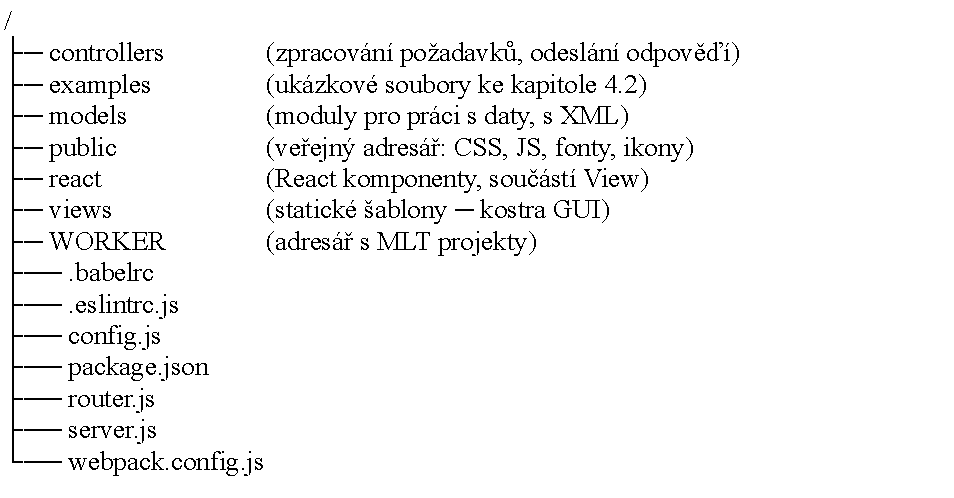
\includegraphics{obrazky-figures/file-structure.pdf}
    }
	\caption{Struktura projektu.}\label{img:structure}
\end{figure}

Významu konfiguračních souborů a souborům v~kořenovém adresáři se budu věnovat v~následujících kapitolách. Jednotlivé části projektu rozebírám v~druhé polovině této kapitoly.

\section{Nastavení, konfigurační soubory}
Po spuštění aplikace se začne vykonávat kód v~souboru \texttt{/server.js}. Nejprve se nastaví prostředí pro zpracovávání požadavků. K~tomu se využívají další soubory -- \texttt{/config.js}, \text{/router.js} a soubory nainstalovaných balíčků.

\subsection{Server}
Soubor \texttt{/server.js} je hlavním souborem projektu. Při spuštění projektu začne interpret Node.js interpretovat právě tento soubor. Soubor má na starost inicializaci prostředí, konkrétně má na starost následující:
\begin{enumerate}
\item Inicializuje JavaScriptový framework \textit{Express}.
\item Inicializuje rozšíření pro zpracování nahrávaných souborů (\textit{busboy}).
\item Inicializuje rozšíření pro zpracování těl požadavků ve formátu \textit{JSON}.
\item Nastaví šablonovací systém, z~pohledu \textit{Express} čisté HTML ve složce \texttt{/views}.
\item Nastaví router na \texttt{/router.js}.
\item Nastaví \texttt{/public} jako veřejný adresář, přístupný ze sítě.
\item Nastaví server, aby naslouchal na portu a adrese uvedené v~souboru \texttt{config.js}.
\end{enumerate}
Tyto činnosti se vykonávají pouze při spuštění serveru. Jakmile se provedou všechny úkony, server naslouchá požadavkům a příchozí požadavky předává routeru.

\subsection{Config\label{cap:config}}
Soubor \texttt{/config.js} je centrem všech konfiguračních direktiv.  Před nasazením v~novém prostředí je nutné hodnoty v~souboru \texttt{/config.js} upravit dle aktuálních údajů. Prvních sedm údajů je závislých na prostředí, ve kterém je plánováno nasazení:
\begin{itemize}
\item \texttt{port} -- číslo portu, na kterém bude server spuštěn. Port musí být volný. Porty s~číslem menším než 1024 mohou vyžadovat oprávnění správce. Výchozí hodnotou je \uv{8080}.
\item \texttt{host} -- doménové jméno. Například \uv{localhost} nebo \uv{eva.fit.vutbr.cz}. Výchozí hodnotou je \uv{localhost}.
\item \texttt{emailServer} -- doménové jméno SMTP serveru pro zasílání emailových upozornění, výchozí hodnotou je \uv{smtp.stud.fit.vutbr.cz}.
\item \texttt{emailPort} -- číslo portu SMTP serveru pro zasílání emailových upozornění, výchozím portem je \uv{465}.
\item \texttt{emailUser} -- uživatelské jméno účtu pro autentizaci na SMTP serveru. Z~tohoto účtu jsou emailová upozornění zasílána. Výchozí hodnotu \uv{xkudla15} je nutné změnit.
\item \texttt{emailPasswd} -- heslo k~účtu pro autentizaci na SMTP serveru. Výchozí hodnota nemá význam.
\item \texttt{adminEmail} -- emailová adresa administrátora. Adresa slouží k~zasílání chyb administrátorovi, ke kontaktování. Výchozí hodnota je \uv{xkudla15@stud.fit.vutbr.cz}.
\end{itemize}

Po konfiguračních direktivách následují funkce \texttt{serverUrl} a \texttt{apiUrl}, které zjednodušují přístup k~adrese napříč projektem. Hodnoty se používají například při vytváření asynchronních požadavků v~React komponentách. Funkce vracejí hodnoty pro protokol HTTP, v~případě nasazení HTTPS je nutné tyto dvě funkce upravit.

Následuje položka \texttt{projectPath}, která udává umístění adresáře s~podadresáři MLT projektů. Podadresáře obsahují jak nahrané soubory, tak i XML soubor pro program MLT. Výchozí hodnotu \uv{WORKER} není nutné měnit, pokud nepotřebujete mít soubory například na jiném disku.

Poslední položkou je objekt \texttt{mapFilterNames}. Objekt slouží k~mapování vlastních názvů filtrů (které nejsou součástí MLT) na názvy filtrů, které jsou součástí MLT. Objekt není nutné upravovat, pokud neimplementujeme další alias pro názvy filtrů.

\subsection{Router}
Routování zajišťuje soubor \texttt{router.js}, který se skládá z~routovacích a middleware pravidel. Pravidla překládají adresu URL na JavaScriptovou funkci (controller), která zajistí obsluhu požadavku. Router z~pohledu architektury MVC též spadá mezi controllery. Routovací pravidlo se obvykle aplikuje první, odpovídající URL požadavku, middleware pravidla se vykonají před routovacími pravidly a pokud v~nich na konci zavoláme funkci \texttt{next}, vykonají se i pravidla následující. Middleware pravidlo používám pro logování všech přístupů, do budoucna i pro autorizaci uživatele. Funkce pro obsluhu požadavku obdrží objekt s~požadavkem, objekt pro budoucí odpověď a funkci \texttt{next}. V~následující ukázce je první pravidlo middleware a druhé je routovací.
\begin{lstlisting}[style=JavaScript]
// Log access
router.use((req, res, next) => {
    console.info(new Date(), ` @ ${req.originalUrl}`);
    next(); // go to the next routes
});
// API route
router.post('/api/project/:projectID/file', apiController.projectFilePOST);
\end{lstlisting}

V~případě, že router nenalezne v~seznamu pravidel odpovídající routovací pravidlo, vrací odpověď s~kódem 404. Tělo odpovědi obsahuje HTML s~textem \uv{Cannot GET /fuu}, pro požadavek metody \uv{GET} a adresou \uv{/fuu}.

Posledním middleware pravidlem je pravidlo pro odchytávání chyb, které  se použije, pokud během řádné obsluhy požadavku dojde k~chybě a je zavolána funkce \texttt{next}. Chybu zpracuje \texttt{errorController}.
\begin{lstlisting}[style=JavaScript]
// Error handling
router.use(errorController.default);
\end{lstlisting}

\subsection{npm}
Soubory \texttt{/package.json} a \texttt{/package-lock.json} slouží k~uložení informací o~projektu. Soubory používá program \textit{npm}. V~souboru \texttt{/package.json} jsou uloženy informace o~projektu, jako je název projektu a popis, verze, GitHub repozitář, informace o~autorovi a licenci, URL pro hlášení chyb a URL stránky projektu. Dále je zde uložen název hlavního JavaScriptového souboru (\texttt{server.js}) a skripty. Například pokud napíšeme v~kořenovém adresáři příkaz \texttt{npm run dev}, použije se příkaz \texttt{./node\_modules/.bin/webpack -wd}.

Nejdůležitější částí souboru je seznam závislostí. Pokud potřebujeme rozšířit funkcionalitu projektu a další funkce, můžeme sáhnout po balíčkovém systému \texttt{npm}\,\footnote{npm -- balíčkový systém pro Node.js, \url{https://www.npmjs.com/}.}. K~22. dubnu 2019 bylo v~systému registrováno téměř 810 tisíc balíčků\,\cite{modulecounts}. Správce \texttt{npm} je výchozí balíčkový systém Node.js, jedná se obdobu správce závislostí \texttt{Composer} pro PHP. Příkazem \texttt{npm install <balicek> --save} provedeme stažení a nainstalování závislosti a zároveň je tato závislost uložena v~souboru \texttt{/package.json}.

Pro zjednodušení soubor \texttt{/package-lock.json} neuvádím ve struktuře projektu. Soubor není pro funkčnost aplikace vyžadován. Pokud soubor neexistuje, \textit{npm} si jej vytvoří. V~tomto souboru je uložen aktuální stav nainstalovaných balíčků, zatímco v~\texttt{/package.json} je seznam balíčků, které \uv{měli} být nainstalovány. Například pokud by měl být nainstalován balíček \texttt{react} ve verzi \textsuperscript{$\wedge$}16.8.6, ve skutečnosti mohl být nainstalován balíček ve verzi 16.8.9. Díky tomu, že závislosti trvají pouze na hlavní verzi, mohou být instalovány nové verze, které jsou zpětně kompatibilní (například opravy chyb).

\section{Zprovoznění projektu}
Pro běh aplikace je nezbytné mít v~systému nainstalované \textit{Node.js}. Postup instalace je uveden na oficiálních stránkách\,\footnote{Oficiální stránky Node.js, \url{https://nodejs.org/en/download/}.}. Aplikace vyžaduje verzi Node.js 8 nebo novější. Nainstalovanou verzi si lze ověřit příkazem \texttt{node --version}. Pro získání závislostí je nutné mít nainstalovaný program \textit{npm}. Měl by být součástí instalace \textit{Node.js}. Nainstalovanou verzi ověříte příkazem \texttt{npm --version}.

Nejprve si projekt zkopírujeme, nebo stáhneme z~repozitáře na Github.com\,\footnote{GitHub repozitář kudlav/videoeditor, \url{https://github.com/kudlav/videoeditor}.} tak, aby adresářová struktura projektu odpovídala obrázku \ref{img:structure}. Adresář, ve kterém se nacházejí soubory projektu dále označuji jako \textit{kořenový adresář} se symbolem \uv{/}. Tímto adresářem se nemyslí kořen souborového systému. Projekt se může nacházet v~libovolném adresáři, pro který máte oprávnění.

Projekt využívá externích závislostí, které nejsou součástí archivu. Některé závislosti jsou závislé na architektuře procesoru. správce závislostí  Seznam závislostí je uveden v~souboru \texttt{package.json}. Stažení všech závislostí provedete příkazem v~kořenovém adresáři \texttt{npm install}.

Před spuštěním je potřeba zkontrolovat a upravit nastavení v~konfiguračním souboru. Popis konfiguračního souboru nabízí kapitola \ref{cap:config}.

Další postup se odvíjí od účelu, za jakým bude server spuštěn. Postup zprovoznění pro účely testování je odlišný od postupu pro produkční nasazení na server. Rozlišení je důležité z~hlediska výkonu a spolehlivosti serveru.

\subsection{Spuštění ve vývojářském režimu}
Pro spuštění se používají 2 následující příkazy.
\begin{lstlisting}[style=bash]
npm run dev-build
npm run dev-start
\end{lstlisting}
První příkaz (\texttt{npm run dev-build}) kompiluje soubor \texttt{views/style.scss} do souboru \texttt{/public/style.css} (kaskádové styly) a také veškerý JavaScript a React komponenty ve složce \texttt{/react} do jednoho souboru: \texttt{/public/main.js}. Po zadání příkazu provede program \textit{Webpack} kompilaci, dokončení je indikováno následujícím výpisem:
\begin{lstlisting}
Version: webpack 4.29.6
Time: 13391ms
Built at: 2019-05-01 12:00:00
...
\end{lstlisting}

V~případě, že plánujeme upravovat soubor \texttt{views/style.scss} nebo soubory ve složce \texttt{/react}, necháme skript dále běžet. Skript bude hlídat soubory a v~případě změny provede novou kompilaci. Pokud soubory neplánujeme upravovat, lze skript po první úspěšné kompilaci ukončit (\texttt{CTR+C}). Webpack lze konfigurovat v~souboru \texttt{/webpack.config.js}. V~souboru se nastavují vstupní a výstupní soubory a pravidla pro konverzi vstupů na výstupy.

Druhým příkazem spustíme server -- \texttt{npm run dev-start}. Server bude běžet, dokud skript neukončíme nebo nedojde k~neošetřené výjimce. Pokud dojde k~chybě, server se zastaví a čeká na změnu souborů. Server lze restartovat ručně zadáním příkazu \texttt{rs}. Při změně JavaScriptových souborů (vyjma složky \texttt{/public}) je server automaticky restartován. Toto chování je dobré na vývoj, ale nevhodné pro produkční nasazení. Kompatibilitu kódu zajišťuje \textit{Babel}, konfiguraci ukládá do souboru \texttt{/.babelrc}.

\subsection{Produkční nasazení}
Při prvním spuštění je nejprve potřeba zkompilovat JavaScriptový soubor, který je zasílán webovému prohlížeči uživatele. Klientský JavaScriptový soubor obsahuje hodnoty z~konfiguračního souboru, proto je nutné provést překompilování zdrojů po každé změně konfigurace. JavaScriptové soubory se pro produkční prostředí liší od těch, generovaných pro testovací sestavení. Zkompilování zdrojů provede následující příkaz:
\begin{lstlisting}[style=bash]
npm run build
\end{lstlisting}

Dále je vhodné nastavit v~prostředí operačního systému proměnnou \texttt{NODE\_ENV}. Díky tomuto nastavení bude \textit{Express} používat cache pro šablony a změní případná chybová hlášení. Dle oficiálních stránek může toto nastavení zvýšit výkon trojnásobně. Proměnnou můžeme nastavit před spuštěním aplikace následujícím příkazem:
\begin{lstlisting}[style=bash]
export NODE_ENV=production
\end{lstlisting}
Další možností je nastavovat proměnnou automaticky při startu systému v~\texttt{/etc/init/env.conf} nebo \texttt{/etc/systemd/system/myservice.service}\,\cite{express}.

Nyní spustíme samotný server (příkaz je alias pro \texttt{npm run start}):
\begin{lstlisting}[style=bash]
npm start
\end{lstlisting}
JavaScriptový kód se spustí ve výchozím režimu kompatibility nástroje \textit{Babel}. Nástroj lze konfigurovat souborem \texttt{/.babelrc}.

\section{Model}
Model je část serveru, která má na starost práci s~daty, operace nad soubory a také poskytuje například emailové služby. Tato část je odstíněna od požadavků a odpovědí, jednotlivé moduly lze používat samostatně, potřebná data se funkcím předají v~parametrech. Funkce mohou, ale nemusí, vracet hodnotu.

Modul \texttt{emailManager} obsahuje funkci \texttt{sendProjectFinished}. Funkce se používá při dokončení renderování výsledného videa. Jako parametry požaduje emailovou adresu příjemce, připadne více adres oddělených čárkou, ID projektu a výsledek zpracování (\texttt{true} pro úspěch, \texttt{false} při chybě). Funkce zasílá emaily skrze SMTP server v~konfiguraci. Aplikace díky tomu nevyžaduje vlastní emailový server. V~případě úspěchu se email zašle pouze vlastníkovi projektu. V~případě, že během zpracování došlo k~chybě, je email zaslán vlastníkovi i administrátorovi. K~odesílání emailů využívám knihovnu \textit{nodemailer}\,\footnote{nodemailer -- npm balíček pro snadné odesílání emailů s~podporou HTML i Unicode, \url{https://github.com/nodemailer/nodemailer}.}.

Modul \texttt{fileManager} má na starost získávání informací o~nahraných souborech. Obsahuje funkci \texttt{getDuration}, která je asynchronní. Funkce vrací \textit{Promise}. V~případě, že se dotážeme na délku video nebo audio souboru, vytvoří se potomek procesu a v~něm se spustí příkaz \textit{FFmpeg} pro zjištění délky média. Jakmile je délka zjištěna, vrací se hodnota funkcí \textit{resolve}. Dotaz na jiný typ souboru vrací hodnotu \texttt{null}. Více o~vytváření procesů v~kapitole \ref{ch:Práce s procesy}.

Modul \texttt{mltxmlManager} usnadňuje práci s~\textit{XML} souborem generovaným pro program \textit{MLT}. Modul má na starost ukládání souboru \texttt{project.mlt}, jako parametry vyžaduje ID projektu a obsah kořenového elementu \texttt{<mlt>} včetně samotného \texttt{<mlt>} tagu. Funkce doplní záhlaví XML a celý řetězec zapíše do souboru projektu. Dále obsahuje funkce na získání relativní cesty k~MLT souboru (\texttt{getMLTpath}) a k~adresáři projektu (\texttt{getWorkerDir}). Zbývající funkce pracují přímo s~XML, zjednodušují například vytváření playlistů nebo tractorů.

Modul \texttt{timeManager} slouží k~práci s~časovými značkami. V~projektu používám pro označení časových okamžiků a k~označení doby trvání čas ve formátu "00:00:00,000", přičemž doba trvání nesmí být nulová. Tento modul obsahuje funkce na sčítání (\texttt{addDuration}) a odčítání času (\texttt{subDuration}) a kontrolu, zda je formát doby trvání validní (\texttt{isValidDuration}). Modul je používán jak na straně serveru, tak v~React komponentách.

\subsection{Import modulů}
Moduly zastřešují související funkce do jednoho celku. Moduly obvykle obsahují proměnné a funkce, které se zpřístupní importováním. Aby bylo možné funkce a proměnné importovat, je nutné v~modulu uvádět klíčové slovo \text{export}. Pokud máme v~modulu více funkcí, musíme uvést, kterou funkci chceme importovat. Při neuvedení se importuje výchozí export. Pokud chceme používat více funkcí jedním importem, je nutné v~modulu veškeré funkce a proměnné obalit do společného objektu, který bude výchozí export. Následující ukázka využívá jednoho hlavního objektu, který je výchozím exportem.
\begin{lstlisting}[style=JavaScript]
export default {
    subDuration(durationA, durationB) {
        // ...
        return subResult;
    },
    addDuration(durationA, durationB) {
        // ...
        return addResult;
    },
    // ...
}
\end{lstlisting}

\subsection{Práce s procesy}\label{ch:Práce s procesy}
Díky událostem a asynchronnímu přístupu k~blokujícím požadavkům není problém čekat na mnohem náročnější operace, než je práce se souborovým systémem. V~projektu je potřeba zpracovávat, konvertovat a získávat informace o~multimédiích. Pro JavaScript například není problém vytvořit potomka, který zpracuje videosoubor, a po skončení potomka pracovat s~jeho výstupem. U~PHP by to byl problém a čekající procesy by mohly způsobit vyčerpání prostředků serveru. Práci s~procesy zpřístupňuje modul Child Processes (\texttt{child\_process}). Z~něj využívám funkci \texttt{exec}, který vytvoří shell a umožní v~něm vykonávat příkazy. Po dokončení posledního příkazu je k~dispozici obsah standardního výstupu a standardního chybového výstupu. Použití příkazu \texttt{exec} demonstruje následující ukázka.
\begin{lstlisting}[style=JavaScript]
exec(`ffmpeg -i ${filepath} 2>&1 | grep Duration | cut -d \' \' -f 4 | sed s/,// | sed s/\\\\./,/`,
    (err, stdout, stderr) => {
        if (err) console.error(err);
        else {
            console.log(stdout.trim());
        }
});
\end{lstlisting}
Funkce \texttt{exec} vytvoří potomka a v~rámci něj získá informaci o~délce souboru \text{filepath}. Délku vypíše v~této ukázce na obrazovku, ale pomocí Promises\,\footnote{Promise -- objekt, který reprezentuje budoucí úspěšné/neúspěšné dokončení asynchronní události a jeho budoucí hodnotu, \url{https://developer.mozilla.org/en-US/docs/Web/JavaScript/Reference/Global_Objects/Promise}.} je možné vytvořit funkci \texttt{getDuration} a délku asynchronně vracet.

Při požadavku na renderování se zkontroluje, zda v~projektu již neexistuje soubor \texttt{processing}. Pro renderování projektu se obdobným způsobem, pomocí \texttt{exec}, volá program \texttt{mlt}. Pokud dojde k~chybě, je odeslán chybový email. Při úspěchu dojde k~zapsání standardního výstupu i chybového výstupu do souborů v~projektu (\texttt{stdout.log} a \texttt{stderr.log}), je odstraněn příznak pro probíhající zpracování (\texttt{processing}) a je odeslán email o~úspěchu.
\begin{lstlisting}[style=JavaScript]
exec(`cd ${projectPath} && melt project.mlt -consumer avformat:output.mp4 acodec=aac
vcodec=libx264 > stdout.log 2> stderr.log`, (err) => {
    if (err) console.error(`exec error: ${err}`);
    fs.unlink(path.join(projectPath, 'processing'), (err) => {
        if (err) console.error(err.stack);
    });
    if (isset(req.body.email)) {
        emailManager.sendProjectFinished(req.body.email, req.params.projectID, !(err));
    }
});
\end{lstlisting}\textbf{}

\subsection{Generování XML}
Se soubory XML se pracuje v~modelu i controlleru. Jelikož se jedná o~práci s~daty, popíšu strukturu generovaných souborů v~této kapitole. Struktura je znázorněna graficky na obrázku \ref{img:schemaXML}.
\begin{figure}[h]
	\centering
	\scalebox{0.6}{
		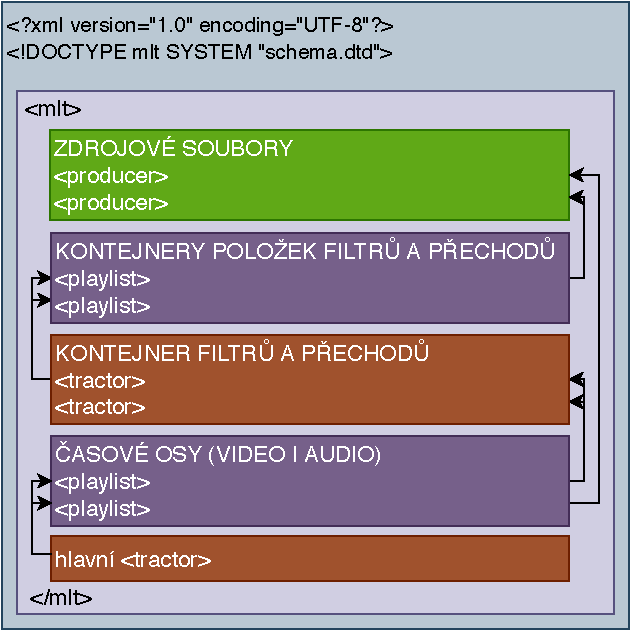
\includegraphics{obrazky-figures/schemaXML.pdf}
	}
	\caption{Obecné schéma prvků generovaných souborů.}\label{img:schemaXML}
\end{figure}

Se založením nového projektu je vytvořen soubor \texttt{project.mlt} obsahující hlavičku XML a odkaz na DTD schéma umístěné v~repozitáři projektu MLT. Poté následuje kořenový tag \texttt{<mlt>}. Uvnitř se nachází jeden playlist pro výchozí stopu \texttt{videotrack0} a hlavní kontejner \texttt{<track>} obsahující odkazy na všechny stopy v~projektu. Tento hlavní kontejner musí být vždy poslední položkou v~kořenovém \texttt{<mlt>}.
\begin{lstlisting}[style=xml]
<?xml version="1.0" encoding="UTF-8"?>
<!DOCTYPE mlt SYSTEM "https://raw.githubusercontent.com/mltframework/mlt/master/src/modu...
<mlt>
    <playlist id="videotrack0"/>
    <tractor id="main">
        <multitrack>
            <track producer="videotrack0" />
        </multitrack>
    </tractor>
</mlt>
\end{lstlisting}

Uvnitř kořenového elementu se nejprve  nacházejí zdrojové soubory (elementy <producer>) u~kterých jsou poznamenány následující vlastnosti -- absolutní cesta k~souboru (\texttt{resource}), typ souboru (\texttt{musecut:mime\_type}), původní název souboru (\texttt{musecut:name}) a v~případě video souboru délka v~milisekundách (\texttt{length}). Zdrojové soubory mají id s~prefixem \uv{producer} a 20 znaky náhodně generovanými při nahrávání souboru.
Po posledním elementu \texttt{<producer>} jsou umístěny pomocné playlisty.

Pomocné playlisty přestavují kontejnery pro položky filtrů a přechodů. Uvnitř těchto playlistů se nachází vždy jedna položka \texttt{<entry>}. Před touto položkou může být v~případě playlistu sloužící pro přechod položka \texttt{<blank>}. Pomocné playlisty jsou identifikovány jako \uv{playlist} a pořadové číslo playlistu. Nové playlisty jsou vkládány na začátek této sekce.

Po playlistech následují tractory (elementy \texttt{<tractor>}). Tyto elementy představují kontejnery pro filtry a přechody. Nesou informace o~aplikovaných filtrech a přechodech. Přechody a filtry aplikují na pomocné playlisty definované výše. Tractor může obsahovat zároveň filtry i přechody. Identifikovány jsou jako \uv{tractor} a pořadové číslo tractoru. Nové tractory jsou vkládány na konec sekce, před stopu s~id \uv{videotrack0};

Předposlední sekcí v~generovaných souborech je část určená stopám. Stopy jsou realizovány jako playlisty. Rozlišují se video a audio stopy. Video stopy jsou identifikovány jako \uv{videotrack} a pořadové číslo video stopy, audio stopy jako \uv{audiotrack} a pořadové číslo audio stopy. Nové stopy jsou vkládány na konec této sekce, před hlavní tractor s~id \uv{main}. Playlisty obsahují posloupnost položek časové osy. Mohou obsahovat \texttt{<entry>} s~odkazem na \texttt{<resource>}, v~případě jednoduché položky, nebo \texttt{<entry>} s~odkazem na \texttt{<tractor>} v~případě aplikovaného filtru nebo přechodu. Mezery mezi položkami řeší vložení elementu \texttt{<blank>} mezi položky.

Posledním elementem v~kořenovém elementu \texttt{<mlt>} musí být vždy hlavní tractor s~id \uv{main}. Tento tractor obsahuje odkaz na všechny stopy. Tento element je pouze jeden a nemůže být smazán. Tento element načítá program \textit{MLT}, z~tohoto elementu jsou skrze odkazy dosažitelné všechny ostatní elementy.

\section{View}
View je část zodpovědná za zobrazení HTML stránek uživateli. Nepoužívám jej při dotazech na API, to je určeno ke strojovému zpracování, ne ke komunikaci s~koncovým uživatelem. View se nachází ve složkách \texttt{/views} a \texttt{/react}. Ve složce \texttt{/views} se nacházejí šablony. Složka \texttt{/react} obsahuje React komponenty.

\subsection{Šablony}
Framework \textit{Express} poskytuje nástroje pro používání různých typů šablon. Protože pro tvorbu uživatelského rozhraní používám React komponenty, zvolil jsem jednoduché HTML soubory. V~těchto soubore je kostra pro namapování React komponent na DOM HTML. V~souborech se rovněž odkazuje na CSS styly a na JavaScriptový soubor, který obsahuje React elementy. Aktuálně se používají 3 šablony -- \texttt{main.html}, \texttt{project.html}, \texttt{finished.html}. Šablona \texttt{main.html} slouží k~zobrazení úvodní obrazovky. Obsahuje přípravu na modální okno pro vytvoření nového projektu. Šablona \texttt{project.html} poskytuje kostru pro stránku s~editorem videa. Šablona \texttt{finished.html} slouží k~zobrazení obrazovky během zpracovávání videa. Stránka se periodicky obnovuje. Pokud si stránky zobrazí uživatel bez zapnutého JavaScriptu, zobrazí se postup řešení problému s~načítáním, obrázek \ref{img:loading-page}.
\begin{figure}[h]
	\centering
	\scalebox{0.9}{
	    
\includegraphics{obrazky-figures/loading-page.pdf}
    }
	\caption{Šablona zobrazená v~prohlížeči s~vypnutým JavaScriptem.}\label{img:loading-page}
\end{figure}

\subsection{React komponenty}
React komponenty používám na úvodní stránce pro vytvoření projektu a na stránce se samotným editorem. Komponenty pro úvodní stránku jsou ve složce \texttt{/react/newProject}, komponenty editory pak ve složce \texttt{/react/editor}.

Na úvodní stránce je kořenovou komponentou třída \texttt{NewProjectDialog}. Třída vykreslí dialog na vytvoření nového projektu. Po stisknutí tlačítka \uv{Vytvořit nový projekt} se pošle požadavek \texttt{POST /api/project}. Pokud API vrátí ID vytvořeného projektu, dojde k~přesměrování na stránku s~editorem. Třída \texttt{NewProjectDialog} je závislá na komponentě \texttt{Modal} z~\textit{npm} balíčku \textit{react-modal}\,\footnote{react-modal -- React komponenta pro vytváření dialogových oken, \url{https://github.com/reactjs/react-modal}.}. Přehled komponent a jejich vzájemných závislostí nabízí obrázek \ref{img:react}.
\begin{figure}[h]
	\centering
	\scalebox{0.7}{
	    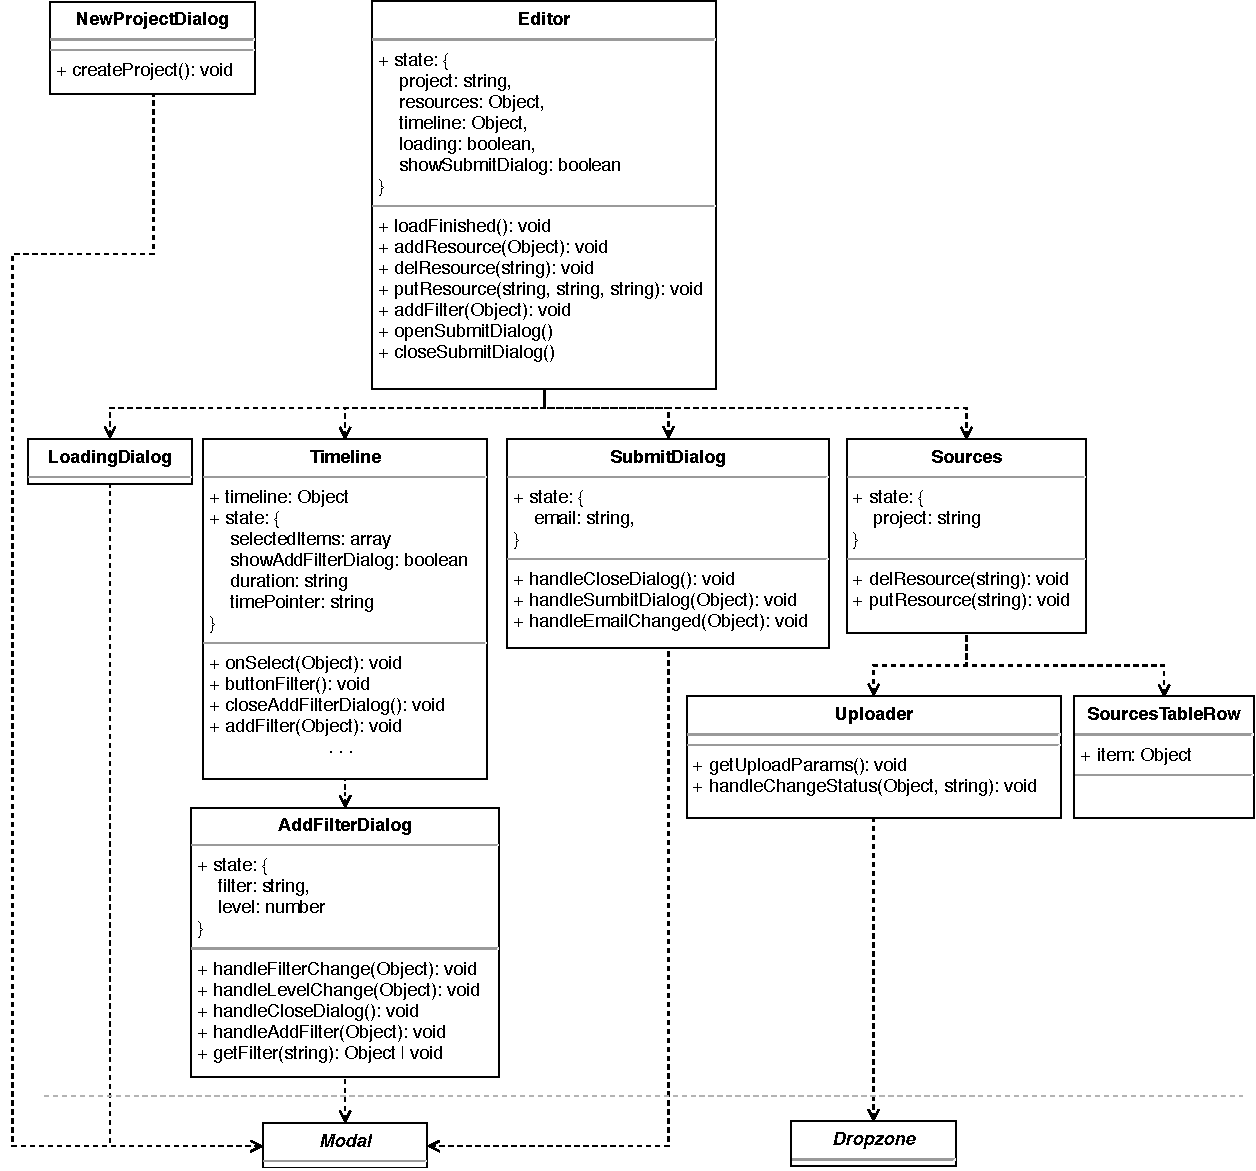
\includegraphics{obrazky-figures/react.pdf}
    }
	\caption{Diagram tříd. Potomci třídy Component s~vyznačením závislostí typu \uv{používání}.}\label{img:react}
\end{figure}

Struktura komponent editoru je rozsáhlejší:

\begin{itemize}
\item \texttt{Editor} je kořenovou komponentou.  Ve svém stavu drží informace o~id projektu, seznam zdrojů projektu a časové osy projektu. Stav projektu získá po načtení stránky z~API požadavkem \texttt{GET /api/project/:projectID}. Poté, co úspěšně získá stav projektu, skryje překryvnou vrstvu s~načítáním. Rovněž řídí viditelnost dialogu pro renderování projektu. Stav projektu propaguje do podřazených komponent \texttt{Timeline} a \texttt{Sources}. Pomocí zpětných volání s~kořenovou komponentou komunikují podřazené komponenty při požadavcích na manipulaci se zdroji a časovou osou.
\item \texttt{SubmitDialog} má na starost dialogové okno pro renderování projektu. Obsahuje formulář pro vyplnění emailu. Po vyplnění emailové adresy a potvrzení zašle na API požadavek \texttt{PUT /api/project/:projectID}. Pokud se vrátí kladná odpověď, je uživatel přesměrován na stránku \texttt{/project/:projectID/finished}.
\item \texttt{Sources} vykresluje seznam zdrojů projektu a formulář pro nahrávání dalších zdrojů. Nahrávání souborů zajišťuje komponenta \texttt{Sources}. Třída \texttt{Sources} používá pro položky zdrojových souborů podřízenou komponentu \texttt{SourcesTableRow}. Pokud podřízené komponenty požádají o~změnu zdrojových souborů / časové osy předá požadavek nadřízené komponentě \texttt{Editor}.
\item \texttt{SourcesTableRow} vykreslí jeden řádek v~seznamu zdrojových souborů. Položka si jako svůj stav udržuje informace o~položce. Položku zdrojů lze přidávat na časovou osu nebo smazat z~projektu. Komponenta volá API -- \texttt{PUT /api/project/:projectID/file/:fileID} pro přidání položky na časovou osu a \texttt{DELETE /api/project/:projectID/file/:fileID} pro smazání souboru. Pokud API vrátí odpověď bez chyby, komponenta požádá nadřazenou komponentu \texttt{Sources} o~změnu zdrojových souborů / časové osy.
\item \texttt{Uploader} slouží k~vykreslení formuláře pro nahrávání souborů. Má za úkol nakonfigurovat komponentu \texttt{Dropzone} z~npm balíčku. Komponentě předá funkce pro zpětná volání při změně stavu (dokončení nahrávání, selhání nahrávání) a tato volání obsluhuje. Při úspěšném nahrání souboru požádá nadřazenou komponentu \texttt{Sources} o~přidání souboru do seznamu zdrojových souborů.
\item \texttt{Timeline} má na starost časovou osu. Časová osa není komponenta React. K~inicializaci časové osy dochází ve funkci \texttt{componentDidMount}, která se volá po umístění komponenty do virtuálního DOM. Při změně položek časové osy dojde k~překreslení pomocí funkce \texttt{componentDidUpdate}. Komponenta má na starost také přidávání filtrů a zobrazování dialogového okna pro přidání filtru -- komponenty \texttt{AddFilterDialog}. Komponenta si ve stavu uchovává pole s~označenými položkami na časové ose a informaci, zda má být viditelné dialogové okno pro přidání filtru. Pokud dialog požádá o~přidání filtru, je požadavek předán nadřazené komponentě \texttt{Editor}.
\item \texttt{AddFilterDialog} vykresluje formulář pro přidání filtru. Ve svém stavu si uchovává hodnoty z~formuláře -- zvolený filtr a jeho hodnotu. Při potvrzení formuláře, komponenta vytvoří objekt flitru a požádá nadřazenou komponentu \texttt{Timeline} o~přidání filtru.
\end{itemize}

\section{Controller}
Controllery mají za úkol přijmout požadavek, zpracovat parametry požadavku, na základě požadavku vykonat s~pomocí modelu požadované akce a poté zajistit odpověď. Odpověď může controller vytvořit sám nebo použije view. Controller je řadič -- řídí ostatní součásti. Složka \texttt{/controllers} obsahuje 3 controllery -- \texttt{apiController}, \texttt{errorController} a \texttt{mainController}.

\subsection{apiController}
Nejrozsáhlejší controller je \texttt{apiController}. Ten nese zodpovědnost za celé API. Má na starost přijímaní požadavků, manipulaci s~XML i vytváření odpovědí. Tento controller nepoužívá view, neboť používám odpovědi pro API výhradně v~jednoduchém formátu \textit{JSON}. Na konci souboru \texttt{apiController} se nacházejí také 3 pomocné funkce -- \texttt{fileErr} (vytvoří odpověď s~chybou čtení projektu), \texttt{isNaturalNumber} (test na nezáporná celá čísla) a \texttt{isset} (kontrola existence proměnných). Tyto funkce jsou pomocné a jsou používány pouze v~rámci souboru.

Nejjednodušším požadavkem je \texttt{GET /api}. Obsluhu zajistí funkce \texttt{default}, která pouze vrátí informaci o~umístění dokumentace k~API. Nejpozději na konci každé hlavní funkce controlleru dojde k~vygenerování odpovědi. V~případě chyby dojde k~vytvoření odpovědi ihned po zaznamenání.

\subsubsection{Vytváření odpovědí}
Každá odpověď obsahuje atribut \texttt{msg}, v~případě úspěchu může obsahovat další položky, v~případě neúspěchu obsahuje odpověď vždy položku \texttt{err} a \texttt{msg}. Jak vypadá odpověď ve funkci \texttt{projectFilePOST}, pokud nepřiložíme nahrávaný soubor, ukazuje následující ukázka.
\begin{lstlisting}[style=JavaScript]
res.status(400);
res.json({
    err: 'Chybi soubor.',
    msg: 'Telo pozadavku musi obsahovat soubor k nahrani.',
});
return;
\end{lstlisting}

V~případě úspěchu chybí položka \texttt{err}, a naopak odpověď obsahuje informace o~nahraném souboru (identifikátor souboru, MIME typ a délku ve formátu \uv{00:00:00,00}).
\begin{lstlisting}[style=JavaScript]
res.json({
    msg: `Upload of "${filename}" OK`,
    resource_id: fileID,
    resource_mime: mimeType,
    length: length,
});
\end{lstlisting}

\subsubsection{Zpracování parametrů požadavku}
Většina funkcí controlleru potřebuje k~činnosti upřesňující parametry HTTP požadavků. Parametry jsou dostupné skrze objekt požadavku (první předávaný parametr). Parametry, které jsou součástí cesty v~URL (projectID, fileID) jsou dostupné skrze \texttt{req.params.projectID}, případně \texttt{req.params.fileID}. Tyto parametry jsou vždy definované. Pokud uživatel parametr v~URL vynechá, router nezavolá obslužnou funkci a zobrazí uživateli chybu 404. V~některých případech by nebylo možné uvádět všechny parametry přímo do URL. Parametry mohou být také v~těle požadavku. K~těmto parametrům se přistupuje pomocí \texttt{req.body.xyz}. Parametry mohou v~požadavku chybět, controller musí na začátku sám ověřit uvedení povinných parametrů funkcí \texttt{isset}.
\begin{lstlisting}[style=JavaScript]
// Required parameters: track, item, filter
if (!isset(req.body.track, req.body.item, req.body.filter)) {
    res.status(400);
    res.json({
        err: 'Chybi parametry.',
        msg: 'Chybi povinne parametry: "track", "item", "filter".',
    });
    return;
}
\end{lstlisting}

Odlišně se přistupuje k~požadavkům během nahrávání souboru. Soubory k~nahrání jsou rovněž uvnitř požadavků jako parametr. Nejsou ve formátu \textit{JSON}, ale \textit{multipart/form-data}. Během nahrávání není potřeba s~daty manipulovat. Při zahájení nahrávání se určí soubor, do kterého se bude zapisovat, a s~dokončením nahrávání vrátí server odpověď o~úspěšnosti operace. K~tomu slouží rozšíření \textit{busboy}. Při přijetí požadavku otestuji, zda obsahuje požadovaná data a poté data přesměruji do souboru.

\subsubsection{Práce s XML}
Serverová část je postavená na práci s~XML. Na parsování XML souborů používám balíček \textit{jsdom}\,\footnote{busboy -- implementace standardů pro práci s~DOM pro Node.js, \url{https://www.npmjs.com/package/jsdom}.}. Node.js neobsahuje nástroje pro práci s~DOM, které jsou v~prohlížečích k~dispozici. Zpracování XML pomocí SAX parseru nepřipadá v~úvahu. SAX parsery procházejí soubory sekvenčně od začátku do konce. DOM přístup umožňuje náhodný přístup k~elementům v~XML dokumentu. Knihovna poskytuje objekt \texttt{window} a \texttt{document}, skrze který jsou dostupné metody známé z~prohlížečů (\texttt{document.getElementById}, \texttt{document.querySelector} apod.). Soubor lze načíst příkazem \texttt{JSDOM.fromFile(mltPath, \{contentType:'text/xml'\})}. Při ukládání lze získat celé XML pomocí atributu \texttt{outerHTML} na kořenový element \texttt{<mlt>} a poté uložit získaný textový řetězec do souboru.

\subsubsection{Práce se souborovým systémem}
Aby mohl controller správně pracovat, potřebuje přístup k~souborům ve složce \texttt{WORKER}. Práci se souborovým systémem umožňuje modul File System (\texttt{fs}). Používání funkcí modulu \texttt{fs} je podobné POSIX funkcím jazyka C. Všechny funkce mají synchronní a asynchronní variantu. U~I/O operací je silně doporučeno používat asynchronní práci se souborovým systémem. Asynchronní funkce mají jako poslední parametr callback, který se zavolá po dokončení operace. Callbacku je jako první parametr předán objekt pro uchování chyb a poté volitelně data operace. Callback je volán při úspěchu i neúspěchu, neúspěch je indikován objektem 1. parametru. Dalším modulem spojeným se souborovým systémem je \texttt{path}, který poskytuje nástroje pro práci s~cestami k~souborům a adresářům. Jak vypadá asynchronní čtení souboru ukazuje následující ukázka.
\begin{lstlisting}[style=JavaScript]
fs.open(path.join(projectPath, 'processing')), 'wx', (err, fd) => {
    if (err) throw err;
    // prace se souborem
    fs.close(fd, (err) => {
        if (err) console.error(err.stack);
    };
});
console.log('stale se muze cekat na nacteni souboru);
\end{lstlisting}

Funkce \texttt{fs.open} je zavolána, vytvoří požadavek souborovému systému a namísto aktivního čekání je funkce uspána a pokračuje se dál vykonáváním příkazů pod \texttt{fs.open}. V~tomto případě by se vypsal do terminálu text \uv{stale se muze cekat na nacteni souboru} a k~práci se souborem by se JavaScriptový engine vrátil až po zpřístupnění požadovaného souboru. Z~toho plyne, že I/O operace jednoho požadavku nebrzdí vykonávání souběžných požadavků.

Pokud chceme moduly použít, je postup jak na straně serveru, tak i na straně klienta (v~React) stejná.
\begin{lstlisting}[style=JavaScript]
import timeManager from '../../models/timeManager';
let actualTime = timeManager.addDuration(timeA, timeB);
\end{lstlisting}

Moduly jsou používány v~rámci jednoho projektu, nejedená se o~\textit{npm} balíčky. Jsou novější alternativou k~používání příkazu \texttt{require}.

\subsubsection{Generování identifikátorů}
Při vytváření nového projektu a při nahrávání souborů je potřeba vygenerovat jednoznačný identifikátor. Generování zajišťuje \texttt{apiController} pomocí balíčku \textit{nanoid}\,\footnote{nanoid -- bezpečný generátor identifikátorů, které mohou být použité v~URL, \url{https://github.com/ai/nanoid}.}. Pro nový projekt se vytváří 32znakový identifikátor, pro nahrávaný soubor generuje 21 znaků. Identifikátory obsahují číslice, velká a malá písmena anglické abecedy a znak podtržítka a spojovníku (A-Za-z0-9\_-). Teoreticky by neměla nastat kolize identifikátorů. Aby byla pravděpodobnost kolize 32znakových identifikátorů 1 \%, museli bychom generovat 1000 identifikátorů za sekundu po dobu větší, než 1 kvadrilion let. V~případě 21znakového identifikátoru souborů bychom museli nahrávat 1000 souborů za sekundu po dobu přibližně 41 milionů let\,\cite{collision}. Součástí projektů mohou být soukromé soubory, které budou chtít uživatelé ochránit před náhodným hádáním ID projektu. Teoreticky je možné procházet všechny možné identifikátory hrubou silou. Hrubou silou by ale bylo možné obejít zabezpečení pomocí uživatelských účtů. Do budoucna se plánuje zkombinovat zabezpečení pomocí ID projektů s~přihlašováním pomocí centrálního autentizačního serveru VUT. Pokud bychom chtěli získat konkrétní projekt hrubou silou, trvalo by nám to opět více než kvadrilion let\,\footnote{K výsledku jsem dospěl na základě kalkulačky na stránkách \url{http://daleswanson.org/things/password.htm} a \url{https://random-ize.com/how-long-to-hack-pass/}}. 

\subsection{errorController}
Pokud dojde během řádné obsluhy požadavku k~výjimce, nebo pokud je zavolána funkce \texttt{next}, předá router obsluhu požadavku controlleru \texttt{errorController}. Tento controller obsahuje pouze funkci \texttt{default}. Dojde k~zalogování chyby a odeslání odpovědi s~chybovým kódem 500 a JSON odpovědí \uv{Internal server error occured.}.
\begin{lstlisting}[style=JavaScript]
exports.default = (err, req, res, next) => {
    console.error(err.stack);
    res.status(500);
    res.json({
        msg: 'Internal server error occured.',
    });
};
\end{lstlisting}

\subsection{mainController}
Controller \texttt{mainController} zpracovává požadavky, u~kterých se očekává odpověď ve formě HTML pro vykreslení webovým prohlížečem. Používá se pro 3 situace. Uživatel navštíví úvodní stránku s~možností vytvořit nový projekt, uživatel zobrazí stránku s~editorem, uživatel zobrazí stránku s~výsledným videem / s~obrazovkou informující o~stavu zpracování. Činnost controlleru je jednoduchá. Při zobrazení úvodní stránky nebo stránky s~projektem controller pouze předá požadavek na vykreslení view.
\begin{lstlisting}[style=JavaScript]
exports.main = (req, res) => res.render('main', {});
\end{lstlisting}

Při požadavku na výsledné video se controller podívá do adresáře projektu po příznaku probíhajícího zpracování (soubor \texttt{processing}). V~případě probíhajícího zpracování požádá view o~vykreslení čekací obrazovky. Pokud se video nezpracovává, podívá se, jestli existuje výsledný soubor \texttt{output.mp4}. Pokud soubor neexistuje, nemá projekt výsledné video a je vrácena chyba 404. Pokud je soubor k~dispozici, zašle se v~odpovědi přímo samotný soubor, odpovědí není HTML stránka.
\begin{lstlisting}[style=JavaScript]
fs.access(path.join(config.projectPath, req.params.projectID, 'processing'), fs.constants.R_OK, (err) => {
    if (err) {
        const outputFile = path.resolve(path.join(config.projectPath, req.params.projectID, 'output.mp4'));
        fs.access(outputFile, fs.constants.R_OK, (err) => {
            if (err) res.sendStatus(404);
            else res.sendFile(outputFile);
        });
    }
    else res.render('finished', {});
});
\end{lstlisting}

\chapter{Testování}
Testování slouží k~odhalení chyb a k~vylepšení uživatelského zážitku. Cíl testování může být různý. Nejprve se v~této kapitole věnuji testování vykreslování (UI) a testování uživatelského zážitku (UX), ve druhé části se zaměřuji na testování modelu a testování stavu aplikace.

\section{Testování uživatelského rozhraní}
Už při návrhu editoru a uživatelského rozhraní jsem navrhované řešení konzultoval s~neprofesionálními uživateli desktopových editorů. Během průzkumu jsem zjišťoval používané filtry a typy přechodů. Nakonec jsem filtry roztřídil do dvou kategorií -- vylepšení a efekty. Zatímco vylepšení mohou zlepšit uživatelský zážitek z~výukového videa, efekty odpoutávají pozornost od sdělení videa. Mezi vylepšení se zařadilo například úprava jasu, kontrastu, odstínu, světlosti, sytosti, ostrosti, vyvážení bílé, otočení a velikost, úprava polohy, ořezání, průhlednost. Mezi nepotřebné efekty se zařadil například sépiový a šedotónový filtr, negativ, rozmazání, posun barev, přidávání kazů do videa apod. Bylo důležité s~uživateli provést toto rozdělení, aby mohly být implementovány pouze efekty zlepšující zážitek z~videa. Omezení výběru filtrů a obecně funkcí vede uživatele k~vytváření kvalitních videí (pro výukové účely).

Pro ověření navrženého rozhraní probíhalo uzavřené testování s~vybranými uživateli. Vybíral jsem uživatele, kteří mají zkušenost s~úpravou videí pomocí desktopových aplikací, ale zároveň tyto editory nepoužívají na profesionální úrovni. Potřeboval jsem uživatele, který zná rámcově práci s~videi, ale zároveň může být při používání editoru nejistý. Volba videa byla na uživatelích, aby se objevily možné problémy s~formáty. Za úkol měli spojit 2 videa a na videa aplikovat alespoň jeden filtr. Během testování byl uživateli k~dispozici tester, testování probíhalo formou pozorování.

Z~hlediska implementace UI bylo během testování odhaleno odlišné vykreslování rozložení prvků při rozlišením větším než 2K. Dále bylo upraveno umisťování dialogových oken a ztmavení obrazovky při zobrazení okna.

Rozložení uživatelského rozhraní přišlo všem testovaným subjektům logické, věděli, kde se co nachází a k~čemu jednotlivé části slouží. Připomínky byly k~zadávání hodnoty filtru. Hodnota obrazových filtrů se nyní zadává posuvníkem, zadávání hodnoty do textového vstupu zůstalo pouze pro dobu trvání. Na řešení uživatelé kritizovaly chybějící funkce, které chyběli z~důvodu nekompletní implementace. S~implementovaným uživatelským rozhraním byli uživatelé spokojení, pravděpodobně díky tomu, že bylo rozhraní implementováno, aby odpovídalo principům klasických editorů (např. \textit{iMovie}).

\section{Testování API}
Základním stupněm testování je použití analyzátoru kódu \textit{ESLint}. ESLint dokáže odhalit syntaktické chyby, časté sémantické chyby v~kódu a dále kontroluje jednotný styl kódu. Kontrolu lze provádět z~kořenového adresáře projektu příkazem \texttt{npx eslint <soubor>}. Kontrolu lze provést nad jedním souborem nebo rekurzivně nad obsahem adresáře. Kontrola nástrojem ESLint má smysl pro složky \texttt{/controllers}, \texttt{/models} a \texttt{/react}. Rozsah kontroly se nastavuje konfiguračním souborem \texttt{.eslintrc.js}.

V~průběhu implementace byla průběžně testována správnost generovaného XML souboru. Soubor byl testován na syntaktickou správnost a správnost dle externího \textit{DTD} souboru. Soubor \textit{DTD} je součástí projektu \textit{MLT} a určuje, jakého obsahu může XML nabývat. Validní soubor XML je základem pro úspěšně vyexportovaný projekt. Kontrolu provádělo automaticky vývojové prostředí \textit{IntelliJ IDEA} a namátkově jsem soubor ověřoval na portálu \textit{TRUUGO}\,\footnote{TRUUGO XML Validator -- bezplatný online XML validátor, včetně podpory externího DTD, \url{https://www.truugo.com/xml_validator/}.}.

Správnost výstupního videa byla kontrolována i vizuálně. Renderování projektu jsem testoval pod 32bitovým Ubuntu 16.04 a pod 64bitovým Ubuntu 18.04. Server \textit{prednasky.com}, na kterém je plánováno nasazení, používá operační systém Ubuntu, proto jsem projekt testoval právě pod tímto operačním systémem.

Při testování jsem se s~menšími obměnami vytvářel následující výstupní video: 1. položka jednoduchá, 2. položka s~přechodem do 3. položky, 3. položka s~aplikovaným filtrem a s~přechody na předchozí i následující 4. položku a poslední 5. položka je bez přechodu, ale s~aplikovaným filtrem, obrázek \ref{img:testcase}.
\begin{figure}[h]
	\centering
	\scalebox{1}{
		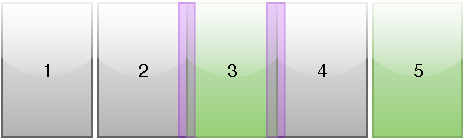
\includegraphics{obrazky-figures/testcase.pdf}
	}
	\caption{Vzorový projekt pro testování. Zelené položky mají aplikován filtr, fialová značí přechod mezi položkami.}\label{img:testcase}
\end{figure}

\section{Rychlost zpracování, maximální délka}
Aby mohlo řešení uživatelům nabídnout lepší služby, než stávající řešení, musí být schopné zpracovat video o~délce delší než 30 minut, ideálně delší než 60 minut, viz srovnání stávajících řešení v~tabulce \ref{tab:prices}.

Testování použitelnosti řešení z~hlediska výkonu a maximální možné délky videa probíhalo na zařízení MacBook Air s~1,3GHz procesorem (turbo až 2,6 GHz) \textit{dual-core Intel Core i5} a 4 GB operační paměti. Komunikace s~vlastním řešením probíhala po lokální síti rychlostí až 300 Mb/s, s~konkurenčními řešeními jsem komunikoval rychlostí až 50 Mb/s. Testy byly voleny tak, aby rychlost sítě nehrála roli.

Během testování jsem zkoušel zpracování videa o~délce 1 hodiny a 40 minut při rozlišení 1280x720 a 30 snímcích za sekundu. Velikost videa byla 333 MB, video bylo kódováno ve formátu H264, audio ve formátu AAC, použitý kontejner byl MPEG-4. Video bylo nahráno na portál, vloženo do časové osy a byl na něj aplikován filtr pro zvýšení jasu. Poté byl projekt vyrenderován.

Nahrávání videa do vlastního řešení proběhlo za necelé 4 minuty. Zpracování videa trvalo 45 minut. Po celou dobu zvládal server odpovídat na požadavky ostatních uživatelů. Druhý testovaný nástroj -- \textit{Clipchamp Create} provádí úpravy na straně prohlížeče. Video bylo po přidání do projektu k~dispozici po 10 sekundách. Renderování videa ovšem trvalo přibližně 2,5 hodiny.

V~porovnání těchto přístupů vyhrává serverové zpracování videí. U~kratších videí se náskok snižuje, ale stále převažuje. Implementované řešení zvládá zpracovat videa delší než 60 minut a překonává tak existující řešení, vyjma \textit{WeVideo} s~neomezenými parametry výsledných videí.

\chapter{Závěr}
V~rámci této práce vznikl REST API server, který slouží k~úpravám multimediálních souborů. K~API je přiložena dokumentace umožňující komukoliv vytvořit vlastní libovolnou aplikaci nad tímto API. K~provozování serveru není zapotřebí databáze ani webový server. K~získávání informací o~souborech používá \textit{FFmpeg}, k~vykreslování výsledného videa framework \textit{MLT}. Server ukládá stav projektů do XML souborů. V~případě potřeby může uživatel editoru znovu načíst projekt ve stavu, v~jakém jej opustil. Také je možné v~libovolném čase vzít složku s~projektem ze serveru a nechat jej ručně zpracovat programem \textit{MLT}. Stačí pouze upravit cesty k~souborům. Zpracování videa není omezeno velikostí souborů ani délkou.

Dále vznikl jednoduchý videoeditor demonstrující základní použití API pro úpravu videí, zejména střih a úpravu záznamů přednášek. Uživatelské rozhraní odpovídá zažitým zvyklostem z~desktopových aplikací. V~současné době umožňuje vkládání videí na časovou osu aplikování filtrů, postupného náběhu a postupného mizení. Uživatelské rozhraní tvoří React komponenty, je tedy snadno rozšiřovatelné. Celá aplikace je tvořena jako open source řešení a zdrojové kódy jsou umístěny na GitHub.com\,\footnote{GitHub repozitář projektu -- dostupný z~\url{https://github.com/kudlav/videoeditor}.} pod licencí Apache-2.0.

Součástí této práce je návod pro zprovoznění řešení pro běžné použití i návod pro sestavení projektu určený budoucím vývojářům. Projekty jsou zabezpečeny unikátním ID. Délka identifikátoru neumožňuje získání konkrétního projektu hrubou silou. Aplikace je dále rozšiřovatelná. Do budoucna se počítá s~rozšířením možností editoru a s~napojením na uživatelské účty na externí autentizační službu.

Dále vznikl ucelený přehled možností manipulace s~multimediálním obsahem přímo v~prohlížeči, včetně ukázek použití pro videoeditor. Efekty nebo přechody je možné simulovat přímo v~prohlížeči, ale samotné renderování výsledného videa je lepší přenechat serverové části.

Tato práce má potenciál pro další rozvoj. Nejvíce prostoru vidím v~možnostech editoru. Zbývá implementovat přechody, některé filtry a náhled videa na základě demonstračních příkladů práce s~videem v~prohlížeči. Konkurenční řešení mají i u~placených programů omezené parametry výsledného videa. Do budoucna vidím možnost zpeněžení nástroje nabídnutím nástroje koncovým uživatelům nebo například online reklamním agenturám.

Za největší přínos považuji vytvoření REST API, díky kterému mohou vzniknout další zajímavé projekty nezávisle na platformě. Může tak vzniknout například nástroj pro úpravu a okamžité sdílení videí s~ostatními uživateli. Se samotným editorem se počítá na portálu \textit{presnasky.com}, kam by měl být nasazen do září 2019.

%===============================================================================

  
  % Kompilace po částech (viz výše, nutno odkomentovat)
  % Compilation piecewise (see above, it is necessary to uncomment it)
  %\subfile{projekt-01-uvod-introduction}
  % ...
  %\subfile{chapters/projekt-05-conclusion}


  % Pouzita literatura / Bibliography
  % ----------------------------------------------
\ifslovak
  \makeatletter
  \def\@openbib@code{\addcontentsline{toc}{chapter}{Literatúra}}
  \makeatother
  \bibliographystyle{bib-styles/slovakiso}
\else
  \ifczech
    \makeatletter
    \def\@openbib@code{\addcontentsline{toc}{chapter}{Literatura}}
    \makeatother
    \bibliographystyle{bib-styles/czechiso}
  \else 
    \makeatletter
    \def\@openbib@code{\addcontentsline{toc}{chapter}{Bibliography}}
    \makeatother
    \bibliographystyle{bib-styles/englishiso}
  %  \bibliographystyle{alpha}
  \fi
\fi
  \begin{flushleft}
  \bibliography{projekt-20-literatura-bibliography}
  \end{flushleft}

  % vynechani stranky v oboustrannem rezimu
  % Skip the page in the two-sided mode
  \iftwoside
    \cleardoublepage
  \fi

  % Prilohy / Appendices
  % ---------------------------------------------
  \appendix
\ifczech
  \renewcommand{\appendixpagename}{Přílohy}
  \renewcommand{\appendixtocname}{Přílohy}
  \renewcommand{\appendixname}{Příloha}
\fi
\ifslovak
  \renewcommand{\appendixpagename}{Prílohy}
  \renewcommand{\appendixtocname}{Prílohy}
  \renewcommand{\appendixname}{Príloha}
\fi
%  \appendixpage

% vynechani stranky v oboustrannem rezimu
% Skip the page in the two-sided mode
%\iftwoside
%  \cleardoublepage
%\fi
  
\ifslovak
%  \section*{Zoznam príloh}
%  \addcontentsline{toc}{section}{Zoznam príloh}
\else
  \ifczech
%    \section*{Seznam příloh}
%    \addcontentsline{toc}{section}{Seznam příloh}
  \else
%    \section*{List of Appendices}
%    \addcontentsline{toc}{section}{List of Appendices}
  \fi
\fi
  \startcontents[chapters]
  \setlength{\parskip}{0pt}
  % seznam příloh / list of appendices
  % \printcontents[chapters]{l}{0}{\setcounter{tocdepth}{2}}
  
  \ifODSAZ
    \setlength{\parskip}{0.5\bigskipamount}
  \else
    \setlength{\parskip}{0pt}
  \fi
  
  % vynechani stranky v oboustrannem rezimu
  \iftwoside
    \cleardoublepage
  \fi
  
  % Přílohy / Appendices
  % Tento soubor nahraďte vlastním souborem s přílohami (nadpisy níže jsou pouze pro příklad)
% This file should be replaced with your file with an appendices (headings below are examples only)

% Umístění obsahu paměťového média do příloh je vhodné konzultovat s vedoucím
% Placing of table of contents of the memory media here should be consulted with a supervisor
%\chapter{Obsah přiloženého paměťového média}

  
  % Kompilace po částech (viz výše, nutno odkomentovat)
  % Compilation piecewise (see above, it is necessary to uncomment it)
  %\subfile{projekt-30-prilohy-appendices}
  
\end{document}
